% =============================================================================
%  MO434 — Deep Learning — Unicamp / Institute of Computing
%  Prof. Dr. Alexandre Xavier Falcao
%  Final Project — A Comparative Study of Knowledge Distillation Schemes
%                  from Pretrained Image Classifiers into a Lightweight ConvNet
%
%  Authors:  Gabriel de Alcantara Bomfim Silveira  (RA 197244)
%            Rodrigo Antonio Godoy de Almeida       (RA 324073)
%
%  Compiler: pdfLaTeX
%  Bib tool: BibTeX  (references.bib)
% =============================================================================
%
% #############################################################################
% ##  READ THIS FIRST — THIS PAPER IS A SCAFFOLD / IMPLEMENTATION GUIDE.      ##
% ##                                                                          ##
% ##  Sections that state DECIDED content (method, definitions, protocol,     ##
% ##  the N=2 Lemma, datasets, setup, figures/tables of the design space) are ##
% ##  written and final. Sections that depend on EXPERIMENTS NOT YET RUN are  ##
% ##  intentionally LEFT BLANK and replaced by boxed/commented guides telling ##
% ##  what to run and how to analyze it. These blanked sections are:          ##
% ##      * Section 7  (Results)      — all subsections                       ##
% ##      * Section 8  (Discussion)   — the results-dependent paragraphs + Q1 ##
% ##      * Section 10 (Conclusion)   — the empirical-conclusion paragraph    ##
% ##  plus the Abstract / Summary headline sentences (marked "% TODO").       ##
% ##                                                                          ##
% ##  Each blank carries: (a) the hypothesis it tests, (b) the exact runs,    ##
% ##  (c) the metrics/instrumentation, (d) the accept/reject analysis rule.   ##
% ##  Fill a blank ONLY with results actually produced; do NOT presuppose a   ##
% ##  positive or negative outcome. The 8 protocol invariants (I1--I8, boxed  ##
% ##  at the top of Section 7) must not be violated.                          ##
% ##                                                                          ##
% ##  A companion file, EXPERIMENTS_EN.md, is the authoritative step-by-step  ##
% ##  execution plan (phases 0--6, staged gating). This .tex mirrors it at    ##
% ##  the points where each result belongs. When in doubt, follow that file.  ##
% #############################################################################
% =============================================================================

\documentclass[11pt,letterpaper]{article}

% -----------------------------------------------------------------------------
%  1. Encoding & language
% -----------------------------------------------------------------------------
\usepackage[utf8]{inputenc}
\usepackage[T1]{fontenc}
\usepackage[english]{babel}
\usepackage{lmodern}                 % vector fonts for screen + print
\usepackage{microtype}               % subliminal typographic polish

% -----------------------------------------------------------------------------
%  2. Page layout
% -----------------------------------------------------------------------------
\usepackage[letterpaper,margin=1in]{geometry}
\usepackage{setspace}
\setstretch{1.10}                    % gentle line spacing
\setlength{\parskip}{0.5\baselineskip}
\setlength{\parindent}{0pt}

% -----------------------------------------------------------------------------
%  3. Headings (titlesec)
% -----------------------------------------------------------------------------
\usepackage{titlesec}
\titleformat{\section}{\large\bfseries}{\thesection}{0.6em}{}
\titleformat{\subsection}{\normalsize\bfseries}{\thesubsection}{0.6em}{}
\titlespacing*{\section}{0pt}{1.4\baselineskip}{0.4\baselineskip}
\titlespacing*{\subsection}{0pt}{1.0\baselineskip}{0.3\baselineskip}

% -----------------------------------------------------------------------------
%  4. Math, figures, tables
% -----------------------------------------------------------------------------
\usepackage{amsmath, amssymb, amsthm}
\newtheorem{theorem}{Lemma}
\usepackage{algorithm}
\usepackage{algpseudocode}
\usepackage{graphicx}
\graphicspath{{figures/}}  % all figures live in a single figures/ folder (Overleaf)
\usepackage{booktabs}
\usepackage{array}
\usepackage{tabularx}
\usepackage{multirow}
\usepackage{caption}
\usepackage{subcaption}
\usepackage{siunitx}                 % nicely aligned numeric columns
\sisetup{detect-weight=true, group-separator={,}, table-number-alignment=center}

% -----------------------------------------------------------------------------
%  5. Lists, colors, hyperlinks, citations
% -----------------------------------------------------------------------------
\usepackage{enumitem}
\setlist{itemsep=2pt, topsep=2pt}
\usepackage{xcolor}
\usepackage{cite}
\usepackage{url}
\usepackage[
    colorlinks=true,
    linkcolor=black,
    citecolor=blue!50!black,
    urlcolor=blue!50!black,
    pdftitle={Graph Relational Knowledge Distillation},
    pdfauthor={Gabriel de Alcantara Bomfim Silveira; Rodrigo Antonio Godoy de Almeida}
]{hyperref}

% -----------------------------------------------------------------------------
%  6. Headers / footers
% -----------------------------------------------------------------------------
\usepackage{fancyhdr}
\pagestyle{fancy}
\fancyhf{}
\fancyhead[L]{\small MO434 \textendash{} Knowledge Distillation Study}
\fancyhead[R]{\small Bomfim \& Almeida}
\fancyfoot[C]{\small \thepage}
\renewcommand{\headrulewidth}{0.4pt}
\renewcommand{\footrulewidth}{0pt}

% -----------------------------------------------------------------------------
%  7. Project metadata (edit here)
% -----------------------------------------------------------------------------
\newcommand{\paperTitle}{Graph Relational Knowledge Distillation: Generalizing Relational KD to Arbitrary-Order Relations}
\newcommand{\authorOne}{Gabriel de Alcantara Bomfim Silveira}
\newcommand{\raOne}{RA: 197244}
\newcommand{\authorTwo}{Rodrigo Antonio Godoy de Almeida}
\newcommand{\raTwo}{RA: 324073}
\newcommand{\submissionDate}{Campinas, 1st semester of 2026}

% =============================================================================
\begin{document}
% =============================================================================

% -----------------------------------------------------------------------------
%  COVER PAGE
% -----------------------------------------------------------------------------
\begin{titlepage}
    \thispagestyle{empty}
    \centering

    {\large \textbf{Universidade Estadual de Campinas (Unicamp)}}\\[0.25cm]
    {\large Institute of Computing}\\[2.0cm]

    {\large MO434 \,\textendash\, Deep Learning}\\[0.25cm]
    {\large Prof. Dr. Alexandre Xavier Falc\~{a}o}\\[2.5cm]

    \rule{0.85\textwidth}{0.4pt}\\[0.6cm]
    {\LARGE \textbf{\paperTitle}}\\[0.6cm]
    \rule{0.85\textwidth}{0.4pt}\\[2.5cm]

    {\large \textbf{Authors}}\\[0.25cm]
    \begin{tabular}{rl}
        \large \authorOne{}  & \large \raOne  \\
        \large \authorTwo{} & \large \raTwo  \\
    \end{tabular}\\[2.5cm]

    \begin{minipage}{0.88\textwidth}
        \small
        \textbf{Summary.} %
        We propose Graph Relational Knowledge Distillation (Graph-RKD), a
        generalization of Relational Knowledge Distillation (RKD) to relations of
        arbitrary order: each minibatch gives rise to several complete, undirected,
        weighted graphs --- one per sampled node set, with the number of nodes set
        by the relational order $N$ --- each summarized by a permutation-invariant
        descriptor (sorted node profiles or the classical-MDS spectrum) and matched
        between teacher and student. We study the method as a design space along
        three axes: the normalization of the graph distance matrix (per-graph,
        minibatch-level, none, and a hybrid scheme), the descriptor, and the
        matching objective (regression and contrastive). The method is implemented
        for deep metric learning (triplet task loss) and evaluated on Stanford
        Cars-196 and CUB-200 with disjoint-class splits, distilling ResNet-18 and
        ConvNeXt-Tiny teachers into a $0.67$M-parameter student. The central
        comparison is Graph-RKD at orders $N \geq 3$ against the distance- and
        angle-wise RKD baselines (RKD-D, RKD-A), all added to the triplet task
        loss under a shared schedule and budget, with the relational weight
        $\lambda_g$ tuned per configuration. We prove that at $N = 2$ the graph
        term either degenerates (under per-graph normalization) or reduces exactly
        to RKD-D (under minibatch normalization), so the pairwise case is
        represented by the RKD-D baseline and Graph-RKD is evaluated only at the
        orders where it is a distinct method. Deriving a rule that predicts the
        quality-optimal $N$ from the minibatch size $K$ is left as future work.
        % TODO: state the headline empirical outcome (Graph-RKD $N\geq3$ vs
        % RKD-D/RKD-A) once the re-tuned, multi-seed experiments are complete.
    \end{minipage}

    \vfill
    \submissionDate
\end{titlepage}

% -----------------------------------------------------------------------------
%  ABSTRACT
% -----------------------------------------------------------------------------
\section*{Abstract}
\addcontentsline{toc}{section}{Abstract}

\noindent
Relational Knowledge Distillation (RKD) transfers the geometry of a teacher's
embedding space by matching pairwise distances and triplet-wise angles, but its
tuple-based formulation is confined to relations of order two and three: the number
of ordered $N$-tuples grows super-exponentially with $N$. We propose Graph
Relational Knowledge Distillation (Graph-RKD), which generalizes relational
transfer to arbitrary order by modeling each minibatch as several complete,
undirected, weighted graphs --- one per sampled node set, whose size is the
relational order $N$ --- whose nodes are examples and whose edge weights are
embedding distances. Because such graphs are determined by their node \emph{sets},
ordering carries no information, reducing the relation space from a falling
factorial to a binomial coefficient; permutation-invariant descriptors (sorted node
profiles or the classical-MDS spectrum) and adaptive graph sampling keep the loss
tractable. We treat Graph-RKD as a design space and study three axes: the
normalization of the graph distance matrix (per-graph, minibatch-level, none, and a
hybrid scheme), the choice of descriptor (profile, MDS), and the matching objective
(regression, contrastive). On fine-grained retrieval (Stanford Cars-196 and
CUB-200, disjoint-class splits), distilling ResNet-18 and ConvNeXt-Tiny teachers
into a $0.67$M-parameter ConvNeXt-inspired student, we compare Graph-RKD at orders
$N \geq 3$ against the distance- and angle-wise RKD baselines (RKD-D, RKD-A), all
added to a triplet task loss under a shared schedule and budget, with the
relational weight tuned per configuration. We show analytically that the pairwise
case $N = 2$ either degenerates under per-graph normalization or reduces exactly to
RKD-D under minibatch normalization, so RKD-D represents that order and Graph-RKD is
evaluated only where it is a distinct method ($N \geq 3$). A methodological finding
recurs throughout: a multi-term distillation loss can zero out \emph{silently},
detectable only by per-term logging. Empirically the outcome is
\emph{dataset-dependent}: on Cars-196 the best-configured Graph-RKD ($N{=}4$, MDS) is the
strongest student while classic pairwise RKD falls \emph{below} the triplet-only floor,
whereas on CUB-200 classic RKD helps and Graph-RKD matches but does not exceed it --- so
higher-order relational transfer is beneficial in some regimes rather than a uniform win
(CUB results are two-seed and provisional). Deriving a rule that predicts the
quality-optimal $N$ from the minibatch size $K$ is outlined as future work.

\bigskip
\hrule
\bigskip

% =============================================================================
%  1. INTRODUCTION
% =============================================================================
\section{Introduction}
\label{sec:introduction}

Modern image classifiers such as VGG~\cite{simonyan2015vgg},
ResNet~\cite{he2016resnet}, and ConvNeXt~\cite{liu2022convnext} share a common
macrostructure: an encoder that produces a spatial feature map, a global average
pooling (GAP) operation that collapses the spatial dimensions, and a linear
classifier. While highly accurate, these backbones are computationally heavy in
both parameter count and inference cost, which limits their deployment on
resource-constrained devices and motivates the search for compact models that
retain the accuracy of their larger counterparts.

Knowledge distillation addresses this need by training a small student network to
imitate a larger pretrained teacher. The paradigm has evolved through several
notions of \emph{what} should be transferred. The seminal formulation of Hinton
et al.~\cite{hinton2015distilling} transfers knowledge at the output level, matching
the teacher's temperature-softened logits. FitNets~\cite{romero2015fitnets} pushes
supervision inward, regressing the teacher's intermediate feature maps, and
Attention Transfer~\cite{zagoruyko2017attention} aligns the spatial attention maps
derived from those activations. All three align \emph{individual} representations,
example by example.

Relational Knowledge Distillation (RKD)~\cite{park2019relational} marked a
conceptual shift: rather than matching the representation of each example in
isolation, it transfers the \emph{mutual relations} between examples --- pairwise
distances and triplet-wise angles in the embedding space. This relational view is
powerful, but the original formulation is confined to relations of order two and
three. Generalizing it to higher-order relations of size $N$ is combinatorially
prohibitive: the number of ordered $N$-tuples drawn from a minibatch grows
super-exponentially with $N$, and much of that count is redundant because the
relational structure of a set of examples does not depend on the order in which
they are listed.

This work proposes \emph{Graph Relational Knowledge Distillation} (Graph-RKD), a
generalization of RKD to relations of arbitrary order. Our central idea is to model
each minibatch as a set of complete, undirected, weighted graphs --- one per sampled
node set, each with $N$ nodes, where the relational order $N$ is a hyperparameter ---
in which every node is an example and every edge weight is the distance between the
embeddings of its endpoints. Because such a graph is fully determined by its
\emph{set} of nodes, the ordering of nodes and edges carries no information, which
removes the redundancy of the tuple formulation and reduces the space of relations
from a falling factorial to a binomial coefficient. To keep the loss tractable even
when this reduced space remains large, we summarize each graph with a
permutation-invariant embedding and train the student over a small set of graphs
sampled afresh at every iteration.
Following the project's suggestion to compare and adapt to the scheme of Park et
al.~\cite{park2019relational}, we instantiate the method in RKD's native
deep-metric-learning setting and evaluate it on two fine-grained retrieval
benchmarks, Stanford Cars-196~\cite{krause2013cars} and
CUB-200~\cite{wah2011cub}, against the distance- and angle-wise RKD variants as
baselines.

The remainder of this paper is organized as follows. Section~\ref{sec:related}
reviews the relevant literature on knowledge distillation, contrastive learning,
and graph representation. Section~\ref{sec:kd-algorithms} formalizes the
distillation algorithms used as baselines. Section~\ref{sec:methodology} presents
the Graph-RKD method, its hypotheses, and its components.
Section~\ref{sec:datasets} describes the datasets,
Section~\ref{sec:setup} the experimental setup, and Section~\ref{sec:results} the
results. Section~\ref{sec:discussion} discusses the findings,
Section~\ref{sec:difficulties} reports the difficulties encountered, and
Section~\ref{sec:conclusion} concludes.

\begin{figure}[t]
    \centering
    \includegraphics[width=0.92\textwidth]{fig_pipeline.pdf}
    \caption{Overview of Graph-RKD. Each minibatch is embedded by the frozen teacher
             and the trained student; the \emph{same} sampled $N$-node node sets are
             turned into complete weighted graphs on both sides, summarized by a
             permutation-invariant descriptor (profile or MDS), and matched by the
             graph loss (regression or contrastive) added to the triplet task loss.
             The descriptor dimensionality depends only on the order $N$, so teacher
             and student spaces of different widths need no projection layer.}
    \label{fig:pipeline}
\end{figure}

% =============================================================================
%  2. RELATED WORK
% =============================================================================
\section{Related Work}
\label{sec:related}

\subsection{Backbone Architectures}
\label{sec:related-backbones}

The teacher and student networks in this work are built from two families of
convolutional backbones. ResNet~\cite{he2016resnet} introduced residual
connections that enable the stable training of very deep networks and remains a
strong, widely used baseline; we adopt its lightweight ResNet-18 variant as one
teacher. ConvNeXt~\cite{liu2022convnext} modernizes the convolutional design with
larger kernels, inverted bottlenecks, and transformer-inspired training recipes,
matching or surpassing vision transformers while retaining a purely convolutional
structure; we use its ConvNeXt-Tiny variant as the second teacher and a compact
ConvNeXt-style network as the student. Both teacher families share the canonical
encoder--GAP--classifier macrostructure, producing a pooled embedding that our
method treats as the node representation of each example.

\subsection{Knowledge Distillation}
\label{sec:related-kd}

The field of knowledge distillation was established by Hinton et
al.~\cite{hinton2015distilling}, who proposed transferring the predictive behavior
of a larger teacher network into a smaller student through softened output
distributions, exposing the relative beliefs across classes encoded in the
temperature-softened logits. Building on this output-level formulation, Romero et
al.~\cite{romero2015fitnets} proposed FitNets, which push supervision earlier in
the network by regressing the teacher's intermediate feature maps through learned
``hint'' layers, while Zagoruyko and Komodakis~\cite{zagoruyko2017attention}
refined this idea by transferring the compact spatial attention maps obtained by
collapsing the channel dimension of those activations. These methods all align
\emph{individual} representations, example by example.

Park et al.~\cite{park2019relational} observed that the preceding approaches share
this single template and proposed Relational Knowledge Distillation (RKD), which
instead transfers the \emph{mutual relations} between examples --- pairwise
distances and triplet-wise angles in the embedding space --- and subsumes the
individual paradigm as its unary special case. RKD is the conceptual foundation of
the present work, and its distance-wise (RKD-D) and angle-wise (RKD-A) losses serve
as our experimental baselines. Logit-based
distillation~\cite{hinton2015distilling} is discussed only as the output-level
origin of the distillation progression, not as a baseline: our metric-learning
setting exposes no shared classifier logits to transfer (Section~\ref{sec:student-config}).
RKD's formulation, however, is confined to relations of order two and
three. Extending it to higher-order relations of size $N$ is combinatorially
prohibitive: the relations are defined over \emph{ordered} tuples, so the number of
distinct tuples grows super-exponentially with $N$, even though the relational
structure of a set of examples is independent of the order in which they are listed.
This scaling barrier is the gap our method addresses.

\subsection{Contrastive and Representation Learning}
\label{sec:related-contrastive}

Contrastive learning maximizes agreement between related views of the data while
separating unrelated ones, a principle formalized by the InfoNCE objective and its
mutual-information bound~\cite{oord2018cpc} and scaled up by
SimCLR~\cite{chen2020simclr} and MoCo~\cite{he2020moco}. The same idea was carried
into distillation by Contrastive Representation Distillation
(CRD)~\cite{tian2020crd}, which pulls the student's representation toward the
teacher's for the same input and pushes it away from others. These objectives trace
back to noise-contrastive estimation~\cite{gutmann2010nce} and the negative-sampling
scheme popularized by word embeddings~\cite{mikolov2013word2vec}. One of our two
distillation objectives adopts this contrastive view, but applies it at the level of
\emph{graph} embeddings rather than individual representations.

\subsection{Graph Learning and Permutation Invariance}
\label{sec:related-graph}

Training over large relational structures by sampling is standard practice in graph
machine learning: GraphSAGE samples fixed-size neighborhoods to learn inductively on
large graphs~\cite{hamilton2017graphsage}, and PinSage scales this strategy to
web-scale recommendation~\cite{ying2018pinsage}. A second requirement, that a
set-level representation be invariant to the ordering of its inputs, is the defining
property of set functions characterized by Deep Sets~\cite{zaheer2017deepsets}. Our
graph descriptors follow both principles: we sample graphs from each minibatch to
keep training tractable, and we summarize each graph with permutation-invariant
embeddings --- one based on sorted node profiles and one on the eigenvalues of the
classical multidimensional-scaling Gram matrix~\cite{torgerson1952mds,cox2000mds},
which are invariant under permutation similarity by construction.

% =============================================================================
%  3. BASELINE DISTILLATION ALGORITHMS
% =============================================================================
\section{Baseline Distillation Algorithms}
\label{sec:kd-algorithms}

This section formalizes the distillation methods against which Graph-RKD is
compared. The distance- and angle-wise variants of Relational
KD~\cite{park2019relational} (RKD-D, RKD-A) are our experimental baselines and are
presented with their loss formulations. Logit-based
distillation~\cite{hinton2015distilling} and the feature-based methods that preceded
RKD are reviewed only as context: the metric-learning setting adopted here exposes no
shared classifier logits to distill, so logit matching is not applicable as a
baseline.

\subsection{Logit-based Distillation (Hinton) --- context}
\label{sec:kd-hinton}

The foundational formulation of knowledge distillation was introduced by Hinton et
al.~\cite{hinton2015distilling}, who proposed transferring the generalization behavior of a
larger teacher network to a smaller student by matching their output distributions. The key
insight is that the soft probabilities produced by the teacher encode rich similarity
structure across classes --- often called \emph{dark knowledge} --- which is lost when
training only with hard labels; both networks apply a temperature-softened softmax, and the
student minimizes a weighted sum of the cross-entropy with the teacher's softened outputs and
a cross-entropy with the true labels. We include this method only as the output-level origin
of the distillation progression: it requires shared classifier logits, which the
metric-learning setting of this work does not provide
(Section~\ref{sec:student-config}), so it is not used as a baseline and we omit its loss
formulation, in parallel with the feature-based methods below.

\subsection{Other Feature-based Methods}
\label{sec:kd-feature}

Between logit matching and relational distillation, two feature-based methods
bridged the gap and are noted here for context, though they are not used as
baselines in our experiments. FitNets~\cite{romero2015fitnets} was the first to
distill knowledge from the teacher's \emph{intermediate} feature maps rather than
its output, using a ``hint'' layer in the teacher to supervise a ``guided'' layer
in the student through a regression objective, with a convolutional regressor
reconciling the differing widths. Attention Transfer~\cite{zagoruyko2017attention}
refined this by transferring not the full feature map but a compact spatial
attention map obtained by collapsing the channel dimension, a more transferable
signal that was the first such method to scale to ImageNet. Both push supervision
into the interior of the network while still aligning individual representations,
the paradigm that Relational KD would subsequently generalize.

\subsection{Relational Knowledge Distillation}
\label{sec:kd-rkd}

Park et al.~\cite{park2019relational} depart from the individual-output paradigm shared by
the preceding methods and propose Relational Knowledge Distillation (RKD), in which the
unit of transferred knowledge is the structure of the embedding space rather than any
single example's representation. Their general formulation (Eq.~\ref{eq:rkd_general})
computes a relational potential $\psi$ over $N$-tuples of examples in both networks and
penalizes the discrepancy between teacher and student potentials, recovering conventional
KD as the unary special case. Two instances are proposed: a distance-wise loss (RKD-D,
Eqs.~\ref{eq:rkd_dist_potential}--\ref{eq:rkd_distance}) that matches pairwise Euclidean
distances normalized by the mean intra-batch distance, and an angle-wise loss (RKD-A,
Eqs.~\ref{eq:rkd_angle_potential}--\ref{eq:rkd_angle}) that matches the cosines of angles
formed by embedding triplets, a higher-order and scale-invariant property that the authors
found to converge faster and perform better. Because relations are invariant to the
dimensionality of individual outputs, RKD requires no projection layer between teacher and
student spaces, in contrast to FitNets~\cite{romero2015fitnets}. The authors emphasize,
however, that relational potentials are blind to absolute output values, so RKD cannot
serve as the sole supervision where individual outputs are the quantity of interest; in
\emph{classification} they combine it with cross-entropy and find it most effective jointly
with logit-based distillation~\cite{hinton2015distilling} --- a combination specific to the
classification setting. In our metric-learning setting there are no shared logits, so RKD-D
and RKD-A are instead added to a triplet task loss (Section~\ref{sec:objectives}). We note
that RKD-A is intrinsically an \emph{order-three} relation (an angle over an example
triplet); Section~\ref{sec:results-order} compares it directly against Graph-RKD at the
matched order $N = 3$, isolating the difference between an angle-based and a distance-based
description of the same three-node structure.

\begin{equation}
    \mathcal{L}_{\text{RKD}} =
    \sum_{(x_1,\ldots,x_n)\in\mathcal{X}^N}
    l\big(\psi(t_1,\ldots,t_n),\, \psi(s_1,\ldots,s_n)\big)
    \label{eq:rkd_general}
\end{equation}

\begin{equation}
    \psi_{\text{D}}(t_i,t_j) = \frac{1}{\mu}\,\lVert t_i - t_j \rVert_2,
    \qquad
    \mu = \frac{1}{|\mathcal{X}^2|}
    \sum_{(x_i,x_j)\in\mathcal{X}^2}\lVert t_i - t_j\rVert_2
    \label{eq:rkd_dist_potential}
\end{equation}

\begin{equation}
    \mathcal{L}_{\text{RKD-D}} =
    \sum_{(x_i,x_j)\in\mathcal{X}^2}
    l_{\delta}\big(\psi_{\text{D}}(t_i,t_j),\, \psi_{\text{D}}(s_i,s_j)\big)
    \label{eq:rkd_distance}
\end{equation}

\begin{equation}
    \psi_{\text{A}}(t_i,t_j,t_k) = \cos\angle t_i t_j t_k
    = \langle \mathbf{e}^{ij}, \mathbf{e}^{kj}\rangle,
    \quad
    \mathbf{e}^{ij} = \frac{t_i - t_j}{\lVert t_i - t_j\rVert_2},
    \;\;
    \mathbf{e}^{kj} = \frac{t_k - t_j}{\lVert t_k - t_j\rVert_2}
    \label{eq:rkd_angle_potential}
\end{equation}

\begin{equation}
    \mathcal{L}_{\text{RKD-A}} =
    \sum_{(x_i,x_j,x_k)\in\mathcal{X}^3}
    l_{\delta}\big(\psi_{\text{A}}(t_i,t_j,t_k),\, \psi_{\text{A}}(s_i,s_j,s_k)\big)
    \label{eq:rkd_angle}
\end{equation}

\noindent
Here $t_i = f_T(x_i)$ and $s_i = f_S(x_i)$ denote the teacher and student representations
of example $x_i$, and $\mathcal{X}^N$ is the set of $N$-tuples of distinct training
examples drawn from the mini-batch. The relational potential function $\psi(\cdot)$
measures a structural property of each tuple, and $l_{\delta}$ denotes the Huber loss,
quadratic for residuals below one and linear beyond, which provides robustness to outlier
relations. The normalization factor $\mu$ in Eq.~\ref{eq:rkd_dist_potential} rescales
distances by their mini-batch mean, making the loss focus on relative structure and
accommodating scale differences between embedding spaces of distinct dimensionality.
Conventional knowledge distillation is recovered from Eq.~\ref{eq:rkd_general} as the
special case $N{=}1$ with $\psi$ the identity, so RKD is a strict generalization of the
individual paradigm. In practice the relational losses are added to a task-specific
objective as $\mathcal{L}_{\text{task}} + \lambda_{\text{KD}}\,\mathcal{L}_{\text{KD}}$,
with one balancing factor per distillation term.

% =============================================================================
%  4. METHODOLOGY  (organized around the 3 phases required by the instructor)
% =============================================================================
\section{Methodology}
\label{sec:methodology}

This section presents Graph Relational Knowledge Distillation (Graph-RKD). We first
describe the overall pipeline and the teacher training stage, then motivate the
method by exposing the scaling limitation of relational distillation, introduce our
graph-based reformulation, and detail each of its components: graph sampling, the
permutation-invariant embeddings, the distillation objectives, and the selection of
the relational order.

\subsection{Overview}
\label{sec:method-overview}

Graph-RKD follows the standard teacher--student distillation setting. A teacher
embedding network is first fine-tuned on the target dataset and then frozen
(Section~\ref{sec:phase-teacher}). A compact student is then trained from scratch
under a combination of a triplet task loss and a \emph{relational graph loss} that
transfers the geometric structure of the teacher's embedding space
(Sections~\ref{sec:tuples-to-graphs}--\ref{sec:order-n}). At each training step the
minibatch is modeled as a set of complete weighted graphs over its examples; both
networks embed the same graphs, and the student is trained to reproduce the
teacher's graph embeddings. At inference time the teacher is discarded: the trained
student produces $L_2$-normalized embeddings that are used directly for retrieval,
with no dependence on the teacher.

\subsection{Teacher Training}
\label{sec:phase-teacher}

The teacher is an ImageNet-pretrained backbone --- ResNet-18 or ConvNeXt-Tiny ---
fine-tuned as an \emph{embedding network} rather than a classifier. Its output is an
$L_2$-normalized embedding, trained with a triplet loss (distance-weighted sampling,
margin $0.2$) on the disjoint training classes, using class-balanced (NPairs)
batches, and evaluated by Recall@K. Once fine-tuning converges, the teacher is
frozen: its parameters are fixed for the entire student distillation stage, and it
is used only to produce reference embeddings. This preserves the pretrained
knowledge while adapting the representation to the metric-learning objective, so the
teacher provides the geometric structure that the student learns to reproduce.

\subsection{From Relational Tuples to Relational Graphs}
\label{sec:tuples-to-graphs}

Relational Knowledge Distillation transfers the mutual relations between examples
rather than their individual representations. In its original form these relations
are defined over \emph{ordered tuples}: pairwise distances over ordered pairs and
angular relations over ordered triples. This formulation has two limitations. First,
it fixes the relational arity to the small constants two and three. Second,
generalizing it to relations of order $N$ is combinatorially prohibitive, because the
number of ordered $N$-tuples drawn without repetition from a minibatch of size $K$ is
the falling factorial
\begin{equation}
    P(K, N) \;=\; \frac{K!}{(K-N)!} \;=\; K (K-1)\cdots(K-N+1),
    \label{eq:falling_factorial}
\end{equation}
which grows super-exponentially in the relational order $N$. Crucially, much of this
count is redundant: the relational structure induced by a set of examples does not
depend on the order in which they are listed.

\subsection{Modeling the Structure as Graphs}
\label{sec:graph-model}

We instead model the relational structure of a minibatch as a \emph{complete,
undirected, weighted graph}, in which each node is an example and each edge weight is
the dissimilarity (distance) between the embeddings of its two endpoints. Because the
graph is complete and undirected, it is fully determined by the \emph{set} of its
nodes, and the ordering of nodes and edges carries no information. The number of
distinct $N$-node graphs that can be formed from a minibatch of size $K$ is therefore
the binomial coefficient
\begin{equation}
    \binom{K}{N} \;=\; \frac{P(K,N)}{N!},
    \label{eq:binomial}
\end{equation}
i.e., a single row of Pascal's triangle. Adopting the set view rather than the tuple
view thus removes a factor of $N!$ --- exactly the orderings that the tuple
formulation counts redundantly. This is the central hypothesis of our method: that
the order-invariant graph is the right object for higher-order relational transfer,
both because it discards redundancy and because it admits the permutation-invariant
descriptors introduced below.

The scale of this redundancy is stark. Figures~\ref{fig:tuples-linear}
and~\ref{fig:graphs-linear} plot, on a linear axis, the number of ordered
$N$-tuples $P(128,N)$ and the number of unique $N$-node graphs $\binom{128}{N}$ for a
minibatch of $K = 128$. On a linear axis both are illegible over the range of
interest: $P(128,N)$ is visually zero until it rises in a near-vertical wall
(it reaches $\approx 3.9\times10^{215}$ at $N=128$), and $\binom{128}{N}$ appears as a
single narrow spike peaking at $N=64$ ($\approx 2.4\times10^{37}$). Only on a
logarithmic axis (Figure~\ref{fig:tuples-vs-graphs}) are both curves readable
simultaneously: the tuple count climbs monotonically while the graph count follows a
symmetric, single-peaked profile, and the vertical distance between them --- the
factor $N!$ removed by the set view --- widens with $N$. We stress that neither space
is enumerable; the set view removes \emph{redundancy} (and yields permutation-invariant
descriptors), not enumeration cost, since both counts are astronomically large.

\begin{figure}[t]
    \centering
    \includegraphics[width=0.72\textwidth]{fig_tuples_linear.pdf}
    \caption{Number of ordered $N$-tuples $P(128,N)$ in a minibatch of $K=128$, linear
             axis. The count is visually indistinguishable from zero across the range
             of practical orders and rises only in a near-vertical wall near $N=128$,
             illustrating why a linear axis is uninformative for this quantity.}
    \label{fig:tuples-linear}
\end{figure}

\begin{figure}[t]
    \centering
    \includegraphics[width=0.72\textwidth]{fig_graphs_linear.pdf}
    \caption{Number of unique $N$-node graphs $\binom{128}{N}$ in a minibatch of
             $K=128$, linear axis. The count is a single symmetric spike peaking at
             $N=K/2=64$ ($\approx 2.4\times10^{37}$) and returning to $1$ at $N=128$;
             on a linear axis the small-$N$ region where the method operates is
             crushed to the baseline.}
    \label{fig:graphs-linear}
\end{figure}

\begin{figure}[t]
    \centering
    \includegraphics[width=0.78\textwidth]{fig_tuples_vs_graphs_log.pdf}
    \caption{Ordered tuples versus unique graphs for $K=128$ on a logarithmic axis.
             Both are legible here: $P(128,N)$ (red) is monotonic and saturating,
             while $\binom{128}{N}$ (blue) is single-peaked and approximately Gaussian
             in $N$ (centered at $N=K/2$, cf.\ Section~\ref{sec:sampling}). The
             vertical gap between the curves equals $\log(N!)$ --- the redundancy the
             set view removes.}
    \label{fig:tuples-vs-graphs}
\end{figure}

\subsection{Tractability through Graph Sampling}
\label{sec:sampling}

The number of distinct graphs is nonetheless very large: $\binom{K}{N}$ is maximized
at $N = K/2$ and reaches astronomical magnitudes (for $K = 128$,
$\binom{128}{64} \approx 2.4 \times 10^{37}$), so enumerating all graphs to evaluate
the loss is infeasible. We make the per-minibatch loss computable by \emph{sampling}
a small set of graphs at each step rather than enumerating them. Each step either
partitions the shuffled minibatch into $\lfloor K/N \rfloor$ node-disjoint graphs or
draws a set of random $N$-node subsets, and the sampled set is re-randomized every
iteration. Under the random-subset scheme the gradient computed over the sample is an
unbiased estimator of the gradient over the full graph space; the partition scheme
trades some of this unbiasedness (it excludes overlapping node sets) for guaranteed
single-pass coverage of every example. Either way the per-step cost is
$O(G \cdot N^2)$ (with $G$ the number of sampled graphs), independent of
$\binom{K}{N}$.

Across a row of Pascal's triangle, $\binom{K}{N}$ is single-peaked and, for large
$K$, approximately Gaussian in $N$ (de Moivre--Laplace~\cite{feller1968probability}), centered at $N = K/2$ with
standard deviation $\sqrt{K}/2$; equivalently $\log\binom{K}{N}$ is approximately
parabolic in $N$ near the peak. This describes the shape of the graph space and
locates its maximum, though the approximation is quantitatively loose in the
small-$N$ tail ($N \ll K/2$) where our experiments operate, so we use it only as a
shape guide, not a quantitative model. Because the graph space varies strongly with
the relational order, we let the number of sampled graphs grow with that size rather
than holding it fixed:
\begin{equation}
    G(N) \;=\; \mathrm{clamp}\!\big(\,\alpha \, \log_2 \tbinom{K}{N},\; g_{\min},\; g_{\max}\big),
    \label{eq:adaptive_sampling}
\end{equation}
with $\alpha = 0.5$ and $g_{\min} = \lfloor K/N \rfloor$ (at least one full-batch
partition, ensuring coverage no worse than node-disjoint sampling), and an optional
cap $g_{\max}$. The two terms are complementary and peak at opposite ends of $N$: the
partition floor $\lfloor K/N \rfloor$ decreases monotonically (dominating at small
$N$, where it guarantees cheap full-batch coverage), while the $\log$-term follows the
Gaussian-like profile of $\binom{K}{N}$ (dominating near $N = K/2$, where the space is
most diverse and a single partition of $\approx 2$ graphs would sample it far too
thinly). We stress that this is a heuristic for matching sample \emph{diversity} to
the space, not a variance-reduction argument: the variance of a Monte-Carlo mean does
not depend on population size. The justification is instead that the per-graph loss is
most \emph{heterogeneous} near $N = K/2$ (graphs there differ most from one another),
so its population variance is largest there, warranting more samples to control the
estimator; $\log_2\binom{K}{N}$ is simply a convenient bounded function that peaks at
$K/2$, and $\alpha$ is a tuning knob. Algorithm~\ref{alg:sampling} summarizes the
procedure.

\begin{algorithm}[htbp]
\caption{Adaptive graph sampling}
\label{alg:sampling}
\begin{algorithmic}[1]
\Require batch size $K$, order $N$, $\alpha$, $g_{\min}$ (default $\lfloor K/N \rfloor$), $g_{\max}$
\State $G \gets \mathrm{round}(\alpha \cdot \log_2 \binom{K}{N})$
\State $G \gets \mathrm{clamp}(G, g_{\min}, g_{\max})$
\State \Return $G$ random $N$-subsets of $\{1, \ldots, K\}$ \Comment{or $\lfloor K/N \rfloor$ disjoint, if partition}
\end{algorithmic}
\end{algorithm}

\subsection{Permutation-Invariant Graph Embeddings}
\label{sec:embeddings}

Each sampled graph is summarized by a fixed-length descriptor computed from its
dissimilarity matrix $D \in \mathbb{R}^{N \times N}$. The descriptor must be invariant
to permutations of the node indexing (relabeling rows and columns of $D$ leaves the
graph unchanged) while remaining sensitive to its structure. We use two such
embeddings.

The \emph{ordered node-profile embedding} sorts the off-diagonal entries of each row
into a per-node neighborhood profile, orders the $N$ profiles lexicographically, and
flattens the result into a vector of size $N(N-1)$. Sorting within each row and then
across nodes destroys the arbitrary node labeling, which is what makes the descriptor
permutation-invariant; the price is that node correspondence (which edge joins which
pair) is discarded, so two structurally different weighted graphs with the same
multiset of sorted profiles collide. The \emph{spectral (classical-MDS) embedding}
applies classical multidimensional scaling: it double-centers the squared
dissimilarity matrix into a Gram matrix
$B = -\tfrac{1}{2}\, J D^{(2)} J$ with $J = I - \tfrac{1}{N}\mathbf{1}\mathbf{1}^\top$,
recovering the inner-product matrix of the point configuration that best reproduces
the distances; its eigenvalues (the squared extents along the principal axes),
sorted in decreasing order, give a descriptor of size $N$ that is invariant under
permutation similarity by construction. Its price is the converse: the spectrum
determines the graph only up to cospectral equivalence, so isospectral graphs
collide. Both descriptors are therefore \emph{lossy} summaries; a small worked
example is instructive: for a three-node graph with normalized edges $(a, b, c)$ the
profile is the sorted-and-flattened list of each node's two incident edges, whereas
the MDS spectrum is the two nonzero eigenvalues of the double-centered
$3 \times 3$ matrix. Table~\ref{tab:descriptor-example} makes this concrete, and also
shows why $N=2$ is excluded: under per-graph normalization the two-node descriptor is
constant regardless of the edge.

\begin{table}[htbp]
    \centering
    \small
    \caption{Worked descriptor examples for small graphs, under per-graph
             normalization (each matrix divided by its own mean off-diagonal entry).
             At $N=2$ the single edge normalizes to $1$, so \emph{both} descriptors are
             constant for every pair --- the degeneration that makes $N=2$ uninformative
             (cf.\ Lemma~\ref{lem:n2}). At $N=3$ the descriptors vary with the (normalized)
             triangle, so the order carries genuine relational signal. Here $\bar d$
             denotes the mean of the three edges and $\hat a=a/\bar d$, etc.}
    \label{tab:descriptor-example}
    \begin{tabularx}{\linewidth}{@{}l l X X@{}}
        \toprule
        Order & Normalized edges & \texttt{profile} (dim $N(N{-}1)$) & \texttt{mds} spectrum (dim $N$) \\
        \midrule
        $N=2$ & $(1)$ & $(1,\,1)$ & $(0.5,\,0)$ \\
        $N=3$ & $(\hat a,\hat b,\hat c)$ & sorted per-node incident-edge pairs & two nonzero eigenvalues of $-\tfrac12 J D^{(2)} J$ \\
        \bottomrule
    \end{tabularx}
\end{table}

\paragraph{Profile versus MDS.} The two descriptors trade off along several axes; at
the feasible orders here ($N \leq 17$) neither is a compute concern (the largest
profile is $272$-dimensional). The \emph{profile} retains every edge weight and is
\emph{operationally interpretable} --- each component is a concrete normalized
distance traceable to a specific example pair, which is precisely the property that
let per-term inspection localize failures --- but its dimension grows as $N(N-1)$, so
its raw loss magnitude is larger and order-dependent, coupling it to the weight
$\lambda_g$ (Section~\ref{sec:objectives}); and its sort introduces non-smoothness at
edge-weight ties. The \emph{MDS} spectrum is compact ($N$-dimensional) and
\emph{theoretically interpretable} (principal-axis variances) but non-local, lossier
(cospectral collisions), and numerically fragile where eigenvalues are near-degenerate.
An offline fidelity/stability probe over random graphs quantifies this last point: the
fraction of MDS spectra with a near-degenerate minimum eigenvalue gap rises from
$\approx 0.1\%$ at $N=3$ to $\approx 12.7\%$ at $N=8$ and $>90\%$ at $N=16,17$ (the
profile's sort-order-tie rate grows more mildly, $\approx 3\%\!\to\!32\%$), which is why
the executed run restricts MDS to the small orders $N \in \{3,4,8\}$
(Section~\ref{sec:setup}). We report both descriptors and let the experiments adjudicate
which transfers better in which regime (Section~\ref{sec:results}).
Table~\ref{tab:descriptor-compare} summarizes the trade-offs.

\begin{table}[htbp]
    \centering
    \small
    \caption{Profile versus MDS descriptor, scoped to the feasible orders
             ($N \leq 17$). Dimensionality is not a compute concern in this regime; its
             only live consequence is the coupling to the loss weight $\lambda_g$.
             Fidelity and explainability move together: the profile keeps the raw edges
             (traceable and less lossy) while MDS compresses to a spectrum (non-local
             and subject to cospectral collisions).}
    \label{tab:descriptor-compare}
    \begin{tabularx}{\linewidth}{@{}l X X@{}}
        \toprule
        Property & \texttt{profile} & \texttt{mds} \\
        \midrule
        Dimension & $N(N{-}1)$ (e.g.\ $272$ at $N{=}17$) & $N$ \\
        Information retained & all edges; loses node correspondence & spectrum only; cospectral collisions \\
        Explainability & operational (per-edge, traceable) & theoretical (principal-axis variances) \\
        $N=2$ reduction (batch norm) & exact RKD-D (linear) & squared-distance variant \\
        Numerical risk & kinks at edge-weight ties & instability at repeated eigenvalues \\
        $\lambda_g$ coupling & stronger (larger raw loss) & milder \\
        \bottomrule
    \end{tabularx}
\end{table}

\paragraph{Normalization of the distance matrix.} Before computing a descriptor, the
graph distance matrix may be rescaled. This normalization is a first-class design axis
of the method, not an incidental step, and we study four schemes: (i) \emph{per-graph}
normalization, dividing each matrix by its own mean off-diagonal entry (making
descriptors scale-invariant and directly comparable between teacher and student of
different embedding widths); (ii) \emph{minibatch-level} normalization, dividing every
graph in a step by the single mean pairwise distance $\mu$ of the whole batch
(Eq.~\ref{eq:rkd_dist_potential}), which preserves cross-graph scale and is the more
stable, lower-variance denominator; (iii) \emph{none} (raw distances), preserving
absolute scale; and (iv) a \emph{hybrid} scheme that uses the $\mu$ of (ii) as the
denominator while keeping the descriptor itself scale-invariant, aiming to recover
both cross-graph scale consistency and teacher/student invariance. Concretely, the
\emph{canonical} hybrid standardizes each descriptor dimension by z-scoring it across
the set of graphs sampled in the step (subtract the per-dimension mean, divide by the
per-dimension standard deviation over the sampled graphs), which applies uniformly to
both the profile and MDS descriptors; at evaluation the standardization statistics are
frozen to their training estimates so the mapping is deterministic. This introduces a
mild dependence on the sampled set, which we prefer to accept in exchange for a single
construction that treats both descriptors identically (keeping the normalization and
descriptor axes separable). As an \emph{MDS-only} ablation we also consider spectrum
ratios (dividing the eigenvalue spectrum by its largest component), a
sample-independent alternative that has no profile analogue and is therefore reported
separately rather than as the default hybrid. A key observation motivates studying all
four: at $N \geq 3$ the schemes are genuinely different objects, not related by a
global constant, so the choice is not cosmetic. Per-graph normalization, moreover,
\emph{degenerates} at $N = 2$: a two-node graph has a single edge, so dividing by its
own mean yields the constant matrix
$\bigl[\begin{smallmatrix}0&1\\1&0\end{smallmatrix}\bigr]$ and hence a constant
descriptor for every pair. Under minibatch normalization, by contrast, the $N = 2$
descriptor recovers exactly the RKD-D potential; we make this precise in
Lemma~\ref{lem:n2} and use it to justify omitting $N = 2$ from the study of Graph-RKD
as a distinct method (Section~\ref{sec:tuples-to-graphs}). Algorithm~\ref{alg:embedding}
details both descriptor variants; the normalization scheme is a parameter of the
\texttt{normalize} step.

\begin{algorithm}[htbp]
\caption{Permutation-invariant graph embedding}
\label{alg:embedding}
\begin{algorithmic}[1]
\Require $D \in \mathbb{R}^{N \times N}$ (distances); method $\in \{\textsc{profile}, \textsc{mds}\}$; normalize
\If{normalize} \Comment{scale-invariance (teacher vs.\ student)}
    \State $D \gets D / \mathrm{mean}_{i \neq j} D_{ij}$
\EndIf
\If{method $=$ \textsc{profile}}
    \For{each row $i$}
        \State $p_i \gets \mathrm{sort\_ascending}(\{ D_{ij} : j \neq i \})$ \Comment{neighborhood profile}
    \EndFor
    \State order $\gets \mathrm{lex\_argsort}(p_1, \ldots, p_N)$ \Comment{canonical node order}
    \State \Return $\mathrm{flatten}([\, p_{\mathrm{order}(1)} ; \ldots ; p_{\mathrm{order}(N)} \,])$ \Comment{in $\mathbb{R}^{N(N-1)}$}
\Else \Comment{\textsc{mds}: classical MDS spectrum}
    \State $J \gets I - \tfrac{1}{N} \mathbf{1}\mathbf{1}^\top$
    \State $B \gets -\tfrac{1}{2}\, J (D \odot D) J$ \Comment{double-centered Gram}
    \State \Return eigenvalues$(B)$ sorted descending \Comment{in $\mathbb{R}^{N}$}
\EndIf
\end{algorithmic}
\end{algorithm}

\begin{theorem}[Graph-RKD reduces to RKD-D at $N=2$]
\label{lem:n2}
Let each two-node graph on examples $(i,j)$ carry the single edge weight
$d_{ij} = \lVert z_i - z_j \rVert_2$, and let normalization be at the minibatch level,
$\tilde{d}_{ij} = d_{ij}/\mu$ with $\mu$ the mean pairwise distance over the batch, so
$\tilde{d}_{ij}$ equals the RKD-D potential $\psi_{\mathrm{D}}$ of
Eq.~\ref{eq:rkd_dist_potential}. Then:
\emph{(i)} the profile descriptor is $g_{ij} = (\tilde{d}_{ij}, \tilde{d}_{ij})$, a
linear bijection of $\tilde{d}_{ij}$, and the regression objective gives
$\lVert g^{s}_{ij} - g^{t}_{ij} \rVert_p = c_p\,|\tilde{d}^{\,s}_{ij} - \tilde{d}^{\,t}_{ij}|$
with $c_1 = 2$, $c_2 = \sqrt{2}$, i.e.\ Graph-RKD coincides with distance-wise RKD up
to a constant absorbed into $\lambda_g$; \emph{(ii)} the MDS descriptor is
$g_{ij} = (\tfrac{1}{2}\tilde{d}_{ij}^{2}, 0)$, matching $\tilde{d}^{2}$ rather than
$\tilde{d}$, a squared-distance variant of RKD-D.
\end{theorem}

\noindent
The equivalence holds per pair and in expectation under full-pair sampling; published
RKD-D uses the Huber potential, so (i) agrees with it in the large-residual regime and
differs only near zero. Under \emph{per-graph} normalization the same $N=2$ cell instead
collapses to a constant descriptor. In every normalization scheme, then, $N = 2$ is
either degenerate or equivalent to RKD-D --- so it carries no information beyond the
RKD-D baseline, and we evaluate Graph-RKD only at the orders $N \geq 3$ where it is a
distinct, higher-order method (Section~\ref{sec:tuples-to-graphs}), with RKD-D serving as
the representative of the pairwise case. A proof is a direct computation on the
$2 \times 2$ matrix and is omitted for brevity.

\subsection{Distillation Objectives}
\label{sec:objectives}

Given the same sampled node set on both sides, we transfer the teacher's relational
geometry to the student through two objectives, both evaluated in this work. The \emph{regression}
objective minimizes the Minkowski distance between the student's and the teacher's
graph embeddings, $\lVert g_s - g_t \rVert_p$, directly matching the teacher's geometry
graph by graph; it is simple and parameter-free. The \emph{contrastive} objective is
an InfoNCE formulation in the spirit of contrastive representation
distillation~\cite{tian2020crd}: the student's embedding of graph $i$ is the anchor,
the teacher's embedding of the same graph $i$ is the positive, and the teacher's
embeddings of other graphs $j \neq i$ provide the negatives, of which $M$ are sampled
per anchor. The loss is the cross-entropy of the resulting $(1{+}M)$-way classification
with the positive as the target, scaled by a temperature $\tau$. This bounds the number
of inter-graph comparisons to $G \cdot M$.

Because the descriptors are deterministic and parameter-free, it is worth stating why a
contrastive objective is well-defined here at all. The descriptor is not learned; the
contrastive loss optimizes the student \emph{network} $f_s$ \emph{through} the
descriptor, whose only requirement is differentiability (sorting is piecewise-linear;
the eigendecomposition has well-defined derivatives away from degeneracies), so gradients
flow back into $f_s$ exactly as under the regression objective. The descriptor plays the
role of a frozen, parameter-free projection head; determinism is orthogonal to gradient
flow. We also temper the usual claim that contrastive transfer is inherently superior:
that argument, imported from settings with no explicit target, is weaker here, since a
regression target exists and the triplet loss already provides representation spreading.
The setup-specific reason contrastive may nonetheless help is that InfoNCE is
similarity-based and therefore scale-normalized, so it should be far less sensitive to
the raw-loss magnitude that couples the regression objective to $\lambda_g$ --- which
makes it most interesting precisely in the regime where a mis-scaled regression weight
fails. Note that the contrastive objective inherits the same $N=2$ degeneration under
per-graph normalization (a constant descriptor makes anchor, positive, and all negatives
coincide), so like regression it is meaningful only at $N \geq 3$ or under
non-degenerate normalization.

In the metric-learning setting both graph objectives are added to a \emph{triplet task
loss} on the student, with a warm-up over the first epochs that ramps a multiplier from
$0$ to $1$ so the relational term reaches its full weight $\lambda_g$ only once the
student's early embeddings are informative; there is no logit-based or cross-entropy
term. The complete distillation step is given in Algorithm~\ref{alg:step}.

\begin{algorithm}[htbp]
\caption{Graph-RKD distillation step (metric learning)}
\label{alg:step}
\begin{algorithmic}[1]
\Require student $f_s$, teacher $f_t$, minibatch $(X, y)$ with class-balanced sampling, order $N$, weight $\lambda_g$, objective $\in \{\textsc{reg}, \textsc{con}\}$, $p$, $M$, $\tau$, epoch $e$, warm-up fraction $w$
\State $Z_s \gets \mathrm{normalize}(f_s.\mathrm{embedding}(X))$ \Comment{$L_2$ embeddings ($B \times d_s$)}
\State $Z_t \gets \mathrm{normalize}(f_t.\mathrm{embedding}(X))$ (no grad) \Comment{$L_2$ embeddings ($B \times d_t$)}
\State $\{ S_1, \ldots, S_G \} \gets$ sample graphs (Algorithm~\ref{alg:sampling})
\For{$g = 1 \ldots G$} \Comment{same node set on both sides}
    \State $e_s[g] \gets \mathrm{GraphEmbedding}(\mathrm{pdist}(Z_s[S_g]))$ \Comment{Algorithm~\ref{alg:embedding}}
    \State $e_t[g] \gets \mathrm{GraphEmbedding}(\mathrm{pdist}(Z_t[S_g]))$ (no grad)
\EndFor
\If{objective $=$ \textsc{reg}}
    \State $\mathcal{L}_{\mathrm{rel}} \gets \mathrm{mean}_g \, \lVert e_s[g] - e_t[g] \rVert_p$
\Else \Comment{contrastive (InfoNCE, CRD-style)}
    \For{$g$}
        \State logits $\gets [\, \mathrm{sim}(e_s[g], e_t[g]),\ \{ \mathrm{sim}(e_s[g], e_t[h]) : h \in \mathrm{negs}(g, M) \} \,] / \tau$
    \EndFor
    \State $\mathcal{L}_{\mathrm{rel}} \gets \mathrm{mean}_g \, \mathrm{CrossEntropy}(\text{logits}, \text{target} = 0)$ \Comment{positive at index 0}
\EndIf
\State $\mathrm{rel} \gets \min(1,\, e / (w \cdot \text{total\_epochs}))$ \Comment{warm-up: balances rel vs.\ triplet}
\State $\mathcal{L} \gets \mathrm{Triplet}(Z_s, y) + \mathrm{rel} \cdot \lambda_g \cdot \mathcal{L}_{\mathrm{rel}}$
\State backprop and update $f_s$
\end{algorithmic}
\end{algorithm}

\noindent
Classic baselines replace $\lambda_g \cdot \mathcal{L}_{\mathrm{rel}}$ by
$\lambda \cdot \mathcal{L}_{\text{RKD-distance}}$ or
$\lambda \cdot \mathcal{L}_{\text{RKD-angle}}$, under the same triplet loss and
warm-up schedule.

\subsection{Choosing the Relational Order \texorpdfstring{$N$}{N}}
\label{sec:order-n}

The relational order $N$ is the central hyperparameter of the method. Its selection
has two distinct parts, which we treat differently.

\paragraph{Compute-budget ceiling (binary search).} The per-step cost under the
partition scheme is $E = K(N-1)/2$ edges, so the largest order that fits a budget $E$
has the closed form
\begin{equation}
    N_{\max} \;\le\; \frac{2E}{K} + 1,
    \label{eq:order_ceiling}
\end{equation}
i.e., the feasible order is inversely proportional to the batch size. Feasibility is a
\emph{monotonic, deterministic} predicate --- if an order $N$ is infeasible, so is
every larger order --- so the ceiling $N_{\max}$ is found exactly by binary search in
$O(\log K)$ evaluations and without any training.

\paragraph{Quality-driven selection (budget-bounded log-spaced sweep).} We
deliberately do \emph{not} use binary search on the validation quality $q(N)$. Binary
search makes an irreversible left/right cut at each midpoint and is valid only when
the search signal is monotonic and noiseless; neither holds here, since $q(N)$ may
rise and then fall (a larger $N$ yields richer relations but fewer graphs per batch
and a harder optimization), and each $q(N)$ is a single, stochastic training estimate.
Instead we evaluate a set of log-spaced candidate orders
\begin{equation}
    \mathcal{C} \;=\; \{\, n_{\min},\; b\,n_{\min},\; b^2 n_{\min},\; \ldots,\; N_{\max} \,\},
    \qquad b = 2,
    \label{eq:order_candidates}
\end{equation}
which contains $\approx \log_b N_{\max}$ points --- the same training budget a binary
search would spend --- but reveals the shape of the quality--$N$ curve without
assuming monotonicity. Following Lemma~\ref{lem:n2}, we omit $N = 2$ (represented by
the RKD-D baseline) and start the sweep at the smallest genuinely higher-order value;
we additionally include $N = 3$ as an explicit candidate --- the arity-matched
counterpart to RKD-A --- even though pure base-$b$ spacing would skip it. Each
candidate is trained with a short schedule over $R$ seeds,
and its score is the mean best validation mAP@R. We then select $N^\ast$ either by
$\arg\max$ or, for parsimony, by the \emph{one-standard-error rule}: the smallest $N$
whose mean score is within one standard error of the best, preferring cheaper
(smaller-$N$) configurations when the difference is not statistically significant. A
final long run is trained at $N^\ast$. This costs $O(R \log_b N_{\max})$ trainings, is
robust to non-monotonic and noisy quality curves, and exposes the curve for
inspection. (The one-standard-error rule is used here only as a conservative
\emph{selection} heuristic on the sweep; reported final metrics use the median and
seed range rather than mean\,$\pm$\,sem, since the seed counts are small ---
Section~\ref{sec:results}.) Beyond selecting a single $N^\ast$, we characterize each
order along convergence speed, seed stability, peak quality, and per-step cost, and
report the order that is best \emph{by trade-off} rather than by peak metric alone.
Algorithm~\ref{alg:order} states the full procedure.

\paragraph{A rule for \texorpdfstring{$N^\ast(K)$}{N*(K)} as future work.} A natural
question is whether the quality-optimal order can be predicted directly from the
minibatch size $K$, as a quality counterpart to the closed-form compute ceiling
$N_{\max} \le 2E/K + 1$. Establishing such a rule would require sweeping $K$ across
datasets, teachers, descriptors, objectives, and normalization schemes --- a
combinatorial program large enough to constitute a separate study --- so we leave it
as future work. The per-order characterization at fixed $K = 128$ produced here is the
groundwork such a study would build on.

\begin{algorithm}[htbp]
\caption{Selecting $N$ (budget-bounded log-spaced sweep)}
\label{alg:order}
\begin{algorithmic}[1]
\Require batch $K$, edge budget $E$, $n_{\min}$, base $b$, seeds $R$, rule $\in \{\textsc{argmax}, \textsc{1se}\}$
\State $N_{\max} \gets$ largest $N$ with $K(N-1)/2 \leq E$ \Comment{$= \lfloor 2E/K + 1 \rfloor$, binary search, no training}
\State $\mathcal{C} \gets \{ n_{\min},\, b\,n_{\min},\, b^2 n_{\min},\, \ldots,\, N_{\max} \}$ \Comment{sorted, unique}
\For{$N \in \mathcal{C}$} \Comment{seed-averaged validation quality}
    \State vals $\gets [\, \mathrm{best\_val\_mAP@R}(\mathrm{distill}(N, \text{short}, \text{seed}=r)) : r = 1 \ldots R \,]$
    \State $\mathrm{mean}[N] \gets \mathrm{mean}(\text{vals})$; \ $\mathrm{sem}[N] \gets \mathrm{std}(\text{vals}) / \sqrt{R}$
\EndFor
\If{rule $=$ \textsc{argmax}}
    \State $N^\ast \gets \arg\max_N \mathrm{mean}[N]$
\Else \Comment{one-standard-error rule}
    \State best $\gets \arg\max_N \mathrm{mean}[N]$
    \State $N^\ast \gets$ smallest $N \in \mathcal{C}$ with $\mathrm{mean}[N] \geq \mathrm{mean}[\text{best}] - \mathrm{sem}[\text{best}]$
\EndIf
\State \Return $N^\ast$ \Comment{final long run trained at $N^\ast$}
\end{algorithmic}
\end{algorithm}

\subsection{Student Architecture}
\label{sec:student-arch}

The student is a compact network built on the design principles introduced by
ConvNeXt~\cite{liu2022convnext} --- larger kernels, inverted bottlenecks, and the
ConvNeXt block structure --- rather than an official ConvNeXt variant; we refer to it
below as the student for brevity. It has stage
dimensions $(24, 48, 96, 192)$ and depths $(1, 1, 3, 1)$, totaling approximately
$0.67$M parameters and $0.11$ GFLOPs at $224 \times 224$ input
(multiply--accumulate convention) --- against $11.69$M parameters\,/\,$1.81$
GFLOPs for ResNet-18 and $28.59$M\,/\,$4.46$ GFLOPs for ConvNeXt-Tiny, i.e., a
$17$--$43\times$ reduction in parameters and $16$--$41\times$ in compute relative
to its teachers. It is trained from scratch
as an embedding network with the combined triplet and graph-loss objective; no
logit-based, attention, or original relational distillation terms are used.

The student's final $L_2$-normalized embedding is $192$-dimensional, against $512$
for ResNet-18 and $768$ for ConvNeXt-Tiny. Because the graph loss compares
permutation-invariant descriptors whose dimensionality depends only on the relational
order $N$, the same descriptor applies unchanged across all three widths: teacher and
student embeddings inhabit the same descriptor space with \emph{no} projection layer
between them, in contrast to FitNets~\cite{romero2015fitnets}, whose learned regressor
exists precisely to reconcile differing widths. A from-scratch student trained with
the triplet loss alone, under identical hyperparameters, serves as an ablation
\emph{floor} --- it measures whether \emph{any} relational term helps over the task
loss alone --- rather than as a comparison target; the comparison of interest is
Graph-RKD against the RKD-D and RKD-A baselines (Section~\ref{sec:student-config}).

% =============================================================================
%  5. DATASETS
% =============================================================================
\section{Datasets}
\label{sec:datasets}

We evaluate on two standard fine-grained deep-metric-learning and retrieval
benchmarks. Stanford Cars-196~\cite{krause2013cars} contains $16{,}185$ images of
$196$ car models, and Caltech-UCSD Birds-200-2011 (CUB-200)~\cite{wah2011cub}
contains $11{,}788$ images of $200$ bird species.

We use the standard \emph{metric-learning split}, in which the training and test
classes are \emph{disjoint}: for Cars-196 the first $98$ classes are used for
training and the remaining $98$ for testing, and analogously the first and last
$100$ classes for CUB-200. This protocol evaluates whether a model has learned to
\emph{measure similarity} rather than to classify a fixed label set, since the test
classes are never seen during training. Because the disjoint split provides no
validation set, we hold out a \emph{class-disjoint} subset of the training classes as
validation: $20\%$ of the training \emph{classes} (selected once by a fixed random
seed, with all images of a held-out class going entirely to validation), so that
validation classes too are unseen during training.
% TODO: report the resulting class and image counts per split for each dataset
% (e.g. a small table: train/val/test classes and images for Cars-196 and CUB-200).

\subsection{Evaluation Metrics}
\label{sec:metrics}

Relevance is binary --- two images match if they share a class --- and we report a
small, purposeful set of retrieval metrics. \textbf{Recall@K} ($K \in \{1,2,4,8\}$)
measures the conventional metric-learning hit rate, i.e., whether a same-class
neighbor appears among the top $K$ retrieved items, and is kept for comparability
with the deep-metric-learning literature. \textbf{R-Precision} and \textbf{mAP@R}
are order-sensitive over all relevant items: for each query they score the full
ranking of its $R$ same-class items rather than only whether one appears in the top
$K$. Following the metric-learning reality check of Musgrave et
al.~\cite{musgrave2020reality}, which shows that Recall@1 is saturated and can be
misleading, \textbf{mAP@R is our primary metric} and the sole model-selection signal
(both the checkpoint and the relational order $N$). Recall@K is retained
\emph{only} for comparability with the deep-metric-learning literature, where it is
the standard, and is reported as a secondary metric --- following Musgrave et al.,
who likewise report but do not rely on it. We omit precision@K, F1@K, nDCG,
and MRR, which add little beyond Recall@K and mAP@R under binary relevance and are
not standard in this setting.

Model selection --- the checkpoint kept for final evaluation and the relational
order $N$ --- relies only on the validation split; the test set is read once, with
the validation-selected checkpoint, and all three metrics (Recall@K, R-Precision,
and mAP@R) are reported on the test split.

\section{Experimental Setup}
\label{sec:setup}

Table~\ref{tab:design-grid} summarizes the experimental design as a grid over the
method's axes, together with the fair-comparison protocol shared by all students.

\begin{table}[htbp]
    \centering
    \small
    \caption{The Graph-RKD experimental design. The method is studied as a grid over
             four axes; the five students share the architecture, teacher, splits,
             budget, task loss, and warm-up schedule, differing only in the relational
             term. Classic baselines use the original RKD weights and recipe; only
             Graph-RKD's $\lambda_g$ is tuned (per configuration, on validation). $N=2$
             is omitted throughout (Lemma~\ref{lem:n2}).}
    \label{tab:design-grid}
    \begin{tabularx}{\textwidth}{l X}
        \toprule
        Axis / factor & Levels \\
        \midrule
        Normalization & per-graph, minibatch-level ($\mu_{\text{batch}}$), none, hybrid \\
        Relational order $N$ & $3, 4, 8, 16, 17$ \ (at $K{=}128$; $N{=}2$ and $N{=}1$ excluded) \\
        Descriptor & \texttt{profile} ($\in\mathbb{R}^{N(N-1)}$), \texttt{mds} ($\in\mathbb{R}^{N}$) \\
        Objective & regression (Minkowski $p{=}2$), contrastive (InfoNCE; $M$, $\tau$) \\
        Dataset $\times$ Teacher & \{Cars-196, CUB-200\} $\times$ \{ResNet-18, ConvNeXt-Tiny\} \\
        \midrule
        Students compared & (1) triplet-only [floor]; (2) +RKD-D; (3) +RKD-A; \\
                          & (4) +RKD-D+RKD-A [1:2]; (5) +Graph-RKD [swept] \\
        Classic weights & RKD-D $=25$, RKD-A $=50$ (prescribed, Huber, $\mu$-norm) \\
        Graph-RKD weight & $\lambda_g$ tuned per configuration on validation \\
        Selection metric & validation mAP@R (Recall@K reported, not selected on) \\
        Final runs & multi-seed headline (2--3 seeds; CUB reached 2), single-seed search phases (seeds not increased); report the \textbf{median} test mAP@R and the median-run checkpoint \\
        \bottomrule
    \end{tabularx}
\end{table}

\subsection{Preprocessing and Data Augmentation}
\label{sec:preprocessing}

All images are processed as $224 \times 224$ RGB tensors. Training uses
\texttt{RandomResizedCrop(224)} followed by a random horizontal flip; at evaluation
(validation and test) we resize the shorter side to $256$ and take a central $224$ crop.
In both cases pixels are scaled to $[0, 1]$ and normalized with ImageNet statistics
(mean $(0.485, 0.456, 0.406)$, std $(0.229, 0.224, 0.225)$), matching the
ImageNet-pretrained teachers. We deliberately do \emph{not} use mixup or cutmix in the
distillation runs: mixing samples would destroy the per-example correspondence that the
graph loss needs to pair student and teacher on identical node sets. Pairwise edge
weights are Euclidean distances between embeddings; the graph distance matrix is then
normalized according to the scheme under evaluation --- per-graph, minibatch-level,
none, or hybrid (Section~\ref{sec:embeddings}) --- rather than by a single fixed rule.

\subsection{Teacher Fine-tuning}
\label{sec:teacher-config}

Teachers are ImageNet-1k pretrained backbones --- ResNet-18 or ConvNeXt-Tiny ---
fine-tuned as \emph{embedding networks} with a triplet loss (distance-weighted
sampling, margin $0.2$) on the disjoint training classes, using $L_2$-normalized
embeddings and class-balanced (NPairs) batches. Checkpoint selection uses validation
mAP@R, consistent with the rest of the pipeline (Section~\ref{sec:metrics}); Recall@K
is additionally reported. Optimization
uses AdamW (lr $10^{-4}$, weight decay $10^{-5}$), $60$ epochs, batch size $128$, a
cosine schedule with a $3$-epoch warm-up, and mixed precision.

\subsection{Student Distillation}
\label{sec:student-config}

The student (Section~\ref{sec:student-arch}) is trained from scratch as
an embedding network with the triplet loss plus the graph loss only --- there is no
Hinton-style logit distillation, since metric learning has no shared classifier logits.
The relational graph term is balanced against the triplet by a warm-up that ramps a
multiplier from $0$ to $1$ over the first $10\%$ of epochs, so the relational term
reaches its full weight $\lambda_g$ only once the student's early embeddings are
informative (the effective weight ramps to $\lambda_g$, not to $1$). Optimization uses
AdamW (lr $10^{-3}$, weight decay $0.05$), a cosine schedule with a $5$-epoch warm-up,
$120$ epochs, batch size $K = 128$, NPairs class-balanced sampling, stochastic depth
$0.1$, and mixed precision.

We compare five students of the same architecture, differing only in the relational
term added to the shared triplet loss and schedule: (1) triplet only, an ablation
\emph{floor}; (2) triplet\,+\,RKD-D; (3) triplet\,+\,RKD-A; (4) triplet\,+\,RKD-D+RKD-A
(the combined classic reference); and (5) triplet\,+\,Graph-RKD, our method, swept over
the normalization, descriptor, objective, and order axes. To represent the classic
baselines at full strength, we follow the original RKD recipe~\cite{park2019relational}:
the distance potential is $\mu$-normalized (Eq.~\ref{eq:rkd_dist_potential}), the
potentials use the Huber loss, and we adopt the paper's prescribed weights --- RKD-D at
$25$, RKD-A at $50$, i.e.\ the original $1{:}2$ distance-to-angle ratio, which the
combined student (4) also uses. These are the weights validated by the baselines'
authors, so no baseline is disadvantaged by our tuning. Graph-RKD, by contrast, has no
prescribed weight, so its $\lambda_g$ is tuned per configuration on the
\emph{validation} split (never on test), and we report its $\lambda_g$-sensitivity so
the chosen value is transparent rather than cherry-picked. All five students share the
teacher, splits, budget, task loss, and warm-up schedule.

\subsection{Graph-Loss Hyperparameters}
\label{sec:graph-config}

Table~\ref{tab:graph-hparams} lists the default configuration of the graph loss. We
evaluate both the \emph{regression} and \emph{contrastive} objectives of
Section~\ref{sec:objectives} across the same grid, and both descriptor variants
(\texttt{profile}, \texttt{mds}) separately; the relational weight $\lambda_g$ is
tuned per configuration on validation rather than fixed. Following Lemma~\ref{lem:n2},
the order sweep omits $N = 2$ (represented by the RKD-D baseline) and runs
$N \in \{4, 8, 16, 17\}$ from the log-spaced schedule plus an explicit $N = 3$ point,
the arity-matched comparison to RKD-A. Under the adaptive sampling rule at $K = 128$,
the effective number of graphs per step is $G = \lfloor K/N \rfloor$ or the
description-length value of Eq.~\ref{eq:adaptive_sampling}, whichever is larger (e.g.
$G = 42, 32, 20, 33, 35$ for $N = 3, 4, 8, 16, 17$).

\begin{table}[htbp]
    \centering
    \small
    \caption{Default graph-loss hyperparameters.}
    \label{tab:graph-hparams}
    \begin{tabularx}{\linewidth}{@{}l X@{}}
        \toprule
        Hyperparameter & Value \\
        \midrule
        edge metric & Euclidean (distance matrix normalization swept: per-graph / minibatch / none / hybrid) \\
        embedding & \texttt{profile} ($\in \mathbb{R}^{N(N-1)}$) or \texttt{mds} ($\in \mathbb{R}^{N}$) \\
        objective & \texttt{regression} (Minkowski, $p=2$) or \texttt{contrastive} (InfoNCE, temp.\ $\tau$) \\
        sampling & adaptive \texttt{log}: $\alpha = 0.5$, $g_{\min} = \lfloor K/N \rfloor$, $g_{\max} = 64$ \\
        loss weight $\lambda_g$ & tuned per configuration on validation (see Section~\ref{sec:student-config}) \\
        relational order $N$ & $\{3, 4, 8, 16, 17\}$ at $K{=}128$ ($N{=}2$ omitted, cf.\ Lemma~\ref{lem:n2}; $N{=}3$ added for RKD-A) \\
        \bottomrule
    \end{tabularx}
\end{table}

\paragraph{Executed configuration.} The table above is the method's full design
space; the run we execute uses a trimmed grid informed by a cheap viability study
(the $\lambda_g$ gate and a design-space probe reusing the teacher). Concretely:
normalization $\in \{\text{per-graph}, \text{minibatch}, \text{none}\}$ (the
\emph{hybrid} scheme was consistently weakest and is dropped); $\lambda_g \in
\{10^{-2}, 10^{-1}, 1\}$ (the usable signal lives at small $\lambda_g$; larger values
fell below the triplet-only floor); and, for the reasons in
Section~\ref{sec:embeddings} (MDS near-degeneracy $>90\%$ at $N \geq 16$),
order $N \in \{3, 4, 8\}$. The search phases (normalization, descriptor, objective)
use a $60$-epoch schedule --- doubled from an initial $30$, at which the undertrained
student sat near the retrieval floor and made selection unreliable --- while the
headline comparison keeps the full $120$-epoch budget.

\section{Results}
\label{sec:results}

% #############################################################################
% ##  FILLED from the trimmed campaign (2026-07). Numbers are median test     ##
% ##  mAP@R, regenerated by RKD/analysis notebooks. Cars-196 n=2-3 seeds;     ##
% ##  CUB-200 n=2 seeds (the third was not run under the time budget) -> CUB  ##
% ##  cells are small-sample and provisional (no significance claim, not      ##
% ##  bolded). The Graph-RKD headline row is the MDS, N=4 configuration.      ##
% #############################################################################

We report results on the trimmed campaign of Section~\ref{sec:setup}. The search
phases (normalization, descriptor, objective) are complete; the headline comparison
has $n{=}2$--$3$ seeds on \textbf{Cars-196} and $n{=}2$ on \textbf{CUB-200} (the third
CUB seed was not run under the project's time budget). Small-sample cells --- CUB in
particular --- are read as \emph{provisional}: with only two seeds we report the median
but make no significance claim and do not bold CUB cells. All figures/values are
median test mAP@R (selection on validation mAP@R, Section~\ref{sec:metrics}); tables
and figures are regenerated from the logged runs by the analysis notebooks
(\texttt{RKD/analysis/}). The central result is \emph{dataset-dependent} and is
reported per (dataset, teacher) cell, never averaged across the two datasets.

\subsection*{Implementation guide: protocol invariants}

% ---- INVARIANTS (do not violate; see also Sections 4--6) --------------------
\noindent\fbox{\parbox{0.97\linewidth}{\small
\textbf{Protocol invariants --- do not violate.} These make the comparison fair.
\begin{itemize}\itemsep2pt
  \item[\textbf{I1}] \textbf{Per-configuration $\lambda_g$ tuning} on \emph{validation}
        (never global, never on test). The original failure was a fixed
        $\lambda_g{=}1000$ calibrated for the tiny $N{=}2$ loss, swamping the triplet
        term $\sim$500:1 at active orders.
  \item[\textbf{I2}] \textbf{Classic baselines at prescribed weights + full RKD recipe}:
        RKD-D $=25$, RKD-A $=50$ (1:2), $\mu$-normalization, Huber potential, RKD
        sampling. Do not re-tune them.
  \item[\textbf{I3}] \textbf{Everything else shared}: teacher, splits, budget, triplet
        task loss, warm-up, optimizer, $K{=}128$. Only the relational term differs.
  \item[\textbf{I4}] \textbf{Selection metric $=$ validation mAP@R} everywhere
        (teacher, student, order). Recall@K reported, never selected on.
  \item[\textbf{I5}] \textbf{Multi-seed finals} reported as the \textbf{median} over
        seeds (not mean\,$\pm$\,sem, which is not meaningful at small $n$). The executed
        campaign reached $n{=}2$--$3$ seeds (Cars) and $n{=}2$ (CUB) under the time
        budget; small-sample cells are flagged as provisional rather than dropped.
  \item[\textbf{I6}] \textbf{Warm-up ramps to $\lambda_g$}, not to 1.
  \item[\textbf{I7}] \textbf{Per-term logging always on}: log \texttt{graph\_loss} and
        \texttt{triplet\_loss} separately every run (a silent zero must be detectable).
  \item[\textbf{I8}] \textbf{No mixup/cutmix} (breaks teacher/student node correspondence).
\end{itemize}
}}

\subsection{Quantitative Results}
\label{sec:results-quant}

% ---- GUIDE: headline comparison (Phase 5) -----------------------------------
% HYPOTHESIS H1 (headline): Graph-RKD at its best (normalization, descriptor,
%   objective, N) matches or exceeds the classic baselines (RKD-D, RKD-A, combined)
%   in test mAP@R, per dataset/teacher. Direction unknown a priori.
%
% RUNS: the five students of Section 6.3 --- (1) triplet-only [floor],
%   (2) +RKD-D, (3) +RKD-A, (4) +RKD-D+RKD-A [1:2], (5) +Graph-RKD [best config] ---
%   full budget (120 ep), >=5 seeds (headline comparison; 3 only as fallback),
%   on {Cars-196, CUB-200} x {ResNet-18, ConvNeXt-Tiny}.
%
% REPORT: Tables of mAP@R (primary) with R-Precision and Recall@{1,2,4,8} (secondary),
%   each as MEDIAN (min-max), n stated, one table per dataset; a grouped bar chart of
%   test mAP@R with the bar at the median and whiskers spanning the seed min-max.
%   Do NOT report mean +/- sem: at n=3 the sem is not meaningful.
%
% ANALYSIS (accept/reject H1) --- range-overlap rule, not sem:
%   - Two configs are distinguishable only if their seed RANGES do not overlap
%     (stricter: every seed of one beats every seed of the other).
%   - ACCEPT "Graph-RKD matches" if its seed range overlaps the best baseline's.
%   - ACCEPT "beats" only if its range lies ENTIRELY ABOVE the best baseline's AND the
%     direction is consistent across both teachers. Report the median difference.
%   - Report per (dataset, teacher). If the direction flips across datasets (as Cars vs
%     CUB did historically), REPORT the flip --- do NOT average it away; it is a
%     finding, not a failure.
Table~\ref{tab:headline} reports the five students' median test mAP@R across the four
cells; Figure~\ref{fig:headline} shows the grouped bars. Graph-RKD here is the chosen
headline configuration (MDS descriptor, $N{=}4$, per-graph normalization,
$\lambda_g{=}0.01$).

\begin{table}[htbp]
    \centering\small
    \caption{Headline (H1): median test mAP@R (\%) of the five students per cell.
             Cars-196 has $n{=}2$--$3$ seeds; CUB-200 has $n{=}2$ (the third seed was
             not run under the time budget, so CUB values are small-sample, provisional
             and not bolded). Graph-RKD $=$ MDS, $N{=}4$, per-graph, $\lambda_g{=}0.01$.
             Best per Cars cell in \textbf{bold}.}
    \label{tab:headline}
    \begin{tabular}{lcccc}
        \toprule
        & Cars\,/\,R18 & Cars\,/\,CvT & CUB\,/\,R18 & CUB\,/\,CvT \\
        \midrule
        triplet-only        & 3.07 & 3.07 & 3.05 & 3.05 \\
        +\,RKD-D            & 1.79 & 2.05 & 3.29 & 2.98 \\
        +\,RKD-A            & 1.93 & 2.29 & 3.50 & 3.07 \\
        +\,RKD-D+RKD-A      & 1.76 & 1.93 & 3.48 & 3.08 \\
        +\,Graph-RKD        & \textbf{3.20} & \textbf{3.35} & 3.12 & 3.08 \\
        \bottomrule
    \end{tabular}
\end{table}

\begin{figure}[htbp]
    \centering
    
\includegraphics[width=0.98\linewidth]{fig_h1_headline.pdf}
    \caption{Median test mAP@R per student, one facet per (dataset, teacher) cell
             (H1). Graph-RKD (blue) is best on both Cars cells; on CUB the classic
             RKD variants are competitive. CUB is two-seed (provisional).}
    \label{fig:headline}
\end{figure}

The result is \textbf{dataset-dependent}. On \textbf{Cars-196}, Graph-RKD is the best
student on both teachers (3.20 / 3.35), and --- strikingly --- the classic RKD variants
fall \emph{below} the triplet-only floor (1.76--2.29 vs 3.07): distance/angle relational
transfer \emph{hurts} on Cars, while the graph term helps. On \textbf{CUB-200} the
regime inverts: classic RKD \emph{helps} (RKD-A best at 3.50 / 3.07, above the 3.05
floor), and Graph-RKD sits above the floor but no higher than the classic variants --- it
trails RKD-A on ResNet-18 (3.12 vs 3.50) and is level with it on ConvNeXt-Tiny (3.08 vs
3.07, where all five students cluster within $\approx$0.1 point). Thus Graph-RKD
\emph{beats classic RKD where RKD hurts (Cars) and does not surpass it where RKD already
helps (CUB)}. The Cars direction is consistent across both teachers; the CUB cells are
two-seed and provisional, so we report them without a significance claim.

\subsection{The Relational Order \texorpdfstring{$N$}{N} and Normalization}
\label{sec:results-order}

% ---- GUIDE: order sweep, viability gate, normalization ablation -------------
% HYPOTHESIS H0 (viability gate, Phase 1): there exists a lambda_g band in which
%   active-order Graph-RKD (N>=3) trains without collapsing to the triplet-only floor.
%   Test on ONE slice first (Cars-196, ResNet-18, profile, regression, minibatch norm,
%   N=4): sweep lambda_g in {1e-2,1e-1,1,10,1e2,1e3}, short schedule, 1-2 seeds.
%   ACCEPT if some lambda_g gives val mAP@R >= floor within noise (record the band).
%   REJECT and STOP if all collapse (~0.002 historically) --- report that as the finding.
%
% HYPOTHESIS H2 (normalization): minibatch or hybrid normalization outperforms
%   per-graph and none at N>=3; hybrid recovers both cross-graph scale AND
%   teacher/student invariance. RUNS: vary norm in {per-graph, minibatch, none,
%   hybrid}, lambda_g re-tuned within each, on N in {3,4,8}. ANALYSIS: ACCEPT where the
%   gap clears noise; for hybrid, additionally verify the invariance property (teacher-mu
%   and student-mu track, or descriptor distributions align), not just accuracy.
%
% PER-ORDER CHARACTERIZATION (feeds H1/H3): for each N in {3,4,8,16,17} report
%   convergence (epochs-to-X%-of-final mAP@R), stability (seed range, collapse count,
%   MDS eigenvalue-gap / profile sort-tie frequency), peak mAP@R, and cost
%   (per-step time, G(N)). Recommend the best-BY-TRADE-OFF N (need not be argmax).
%
% N=2 IS NOT RUN: Lemma (Section 4.6) shows it degenerates (per-graph) or reduces to
%   RKD-D (minibatch); RKD-D represents the pairwise case.
\paragraph{H0 --- viability gate.} On the gate slice (Cars-196 / ResNet-18 / profile /
regression / minibatch / $N{=}4$), validation mAP@R vs $\lambda_g$
(Figure~\ref{fig:h0}) shows a viable band only at \emph{small} $\lambda_g$: at
$\lambda_g{=}0.01$ Graph-RKD sits above the triplet-only floor (validation mAP@R 2.80
vs 2.32), while every $\lambda_g \geq 0.1$ falls below it and degrades monotonically
(1.70 at $0.1$, 1.12 at $1$, down to $\approx$0.8 at $\lambda_g{=}1000$). A
longer-schedule convergence check (80 epochs) confirmed the edge \emph{survives
training} --- Graph-RKD beat the floor by $\sim$14--18\% test mAP@R --- so H0 is
accepted (marginally) and the full grid uses $\lambda_g \in \{0.01, 0.1, 1\}$.

\begin{figure}[htbp]
    \centering
    
\includegraphics[width=0.6\linewidth]{fig_h0_lambda.pdf}
    \caption{H0 gate: validation mAP@R vs $\lambda_g$ (log axis) with the triplet-only
             floor. Only small $\lambda_g$ ($\approx$0.01) stays at/above the floor.}
    \label{fig:h0}
\end{figure}

\paragraph{H2 --- normalization.} At the best $\lambda_g$ ($=0.01$), \emph{per-graph}
and \emph{minibatch} normalization are essentially tied (median test mAP@R 2.34 vs 2.32
at $N{=}3$, 2.36 vs 2.33 at $N{=}4$) and both beat \emph{none}, whose deficit widens with
order as it destabilizes (2.19 at $N{=}3$ down to 1.03 at $N{=}8$); the \emph{hybrid}
scheme, weakest in the design-space probe, was dropped from the full run
(Section~\ref{sec:setup}). Figure~\ref{fig:h2} shows the ablation. We carry
\emph{per-graph} forward as the headline normalization.

\begin{figure}[htbp]
    \centering
    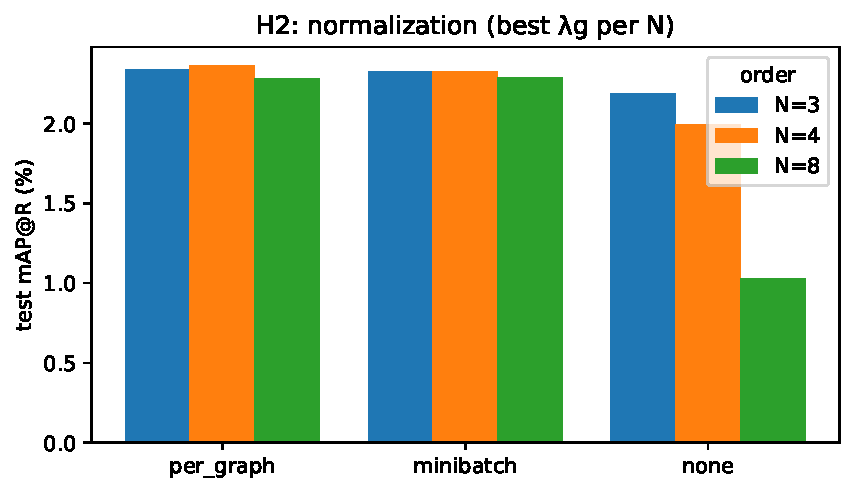
\includegraphics[width=0.6\linewidth]{fig_h2_norm.pdf}
    \caption{H2: median test mAP@R by normalization scheme (best $\lambda_g$ per scheme).
             per-graph $\approx$ minibatch $\gg$ none; hybrid dropped (see text).}
    \label{fig:h2}
\end{figure}

\paragraph{Per-order.} Over the executed orders $N \in \{3,4,8\}$ (60-epoch search
budget, median aggregated across the four cells) test mAP@R decreases with $N$ (MDS:
2.18 / 2.01 / 1.75; profile: 2.03 / 2.01 / 1.57 at $N{=}3/4/8$), so low orders are the
quality-by-cost sweet spot; we adopt $N{=}4$ for the headline. Orders $N \in \{16,17\}$ were excluded because the MDS
spectrum is $>$90\% near-degenerate there (Section~\ref{sec:embeddings}). $N{=}2$ is
excluded by Lemma~\ref{lem:n2}.

\subsection{Descriptor and Objective Characterization}
\label{sec:results-axes}

% ---- GUIDE: profile vs MDS (H3), regression vs contrastive (H4) -------------
% HYPOTHESIS H3 (descriptor): profile and MDS differ in accuracy, stability, and
%   fidelity in characterizable ways; one is preferable in identifiable regimes.
%   RUNS: both descriptors across N in {3,4,8,16,17}, both datasets/teachers, best norm.
%   INSTRUMENT: MDS eigenvalue-gap / near-degeneracy counts and gradient spikes;
%   profile edge-tie frequency; descriptor collision probes (fraction of distinct
%   graphs whose descriptors are within epsilon). ANALYSIS: build a per-scenario table
%   (profile vs MDS mAP@R by N/dataset/teacher); ACCEPT a recommendation only where the
%   accuracy gap clears noise AND is explained by a measured mechanism
%   (stability/fidelity), not a raw number alone.
%
% HYPOTHESIS H4 (objective): the contrastive objective is more robust to lambda_g
%   mis-scaling than regression, because InfoNCE is scale-normalized. RUNS: overlay
%   val mAP@R vs lambda_g for regression and contrastive at a fixed active-order cell.
%   ANALYSIS: ACCEPT if regression shows a sharp peak (collapses outside a narrow band)
%   while contrastive stays within noise of its own best across a much wider lambda_g
%   range; QUANTIFY the width of that range. Also report raw-loss magnitude vs
%   N/descriptor (explains regression's scale sensitivity) and contrastive
%   negative-quality diagnostics (node-overlap contamination; anchor-pos vs anchor-neg
%   similarity gap) to rule out an easy-negatives artifact.
\paragraph{H3 --- descriptor.} On accuracy, profile and MDS are close across the
executed orders (median test mAP@R at the 60-epoch search budget: MDS 2.18 / 2.01 / 1.75
vs profile 2.03 / 2.01 / 1.57 at $N{=}3/4/8$), with MDS marginally ahead at $N{=}3,8$ and
level at $N{=}4$ --- a gap well inside the run-to-run noise at these single-config points,
so we do not claim a winner on accuracy alone. The clean separation is on the \emph{mechanism}: the offline
fidelity/stability probe (Figure~\ref{fig:h3}) shows MDS spectra become $>$90\%
near-degenerate at $N{=}16,17$ (0.1\% at $N{=}3$), while the profile's sort-order-tie
rate grows only mildly. Both descriptors are therefore safe at the small orders we use;
MDS is the headline descriptor (marginally higher accuracy, numerically fine at
$N{\leq}8$), and its instability is the reason large-$N$ MDS is not run.

\begin{figure}[htbp]
    \centering
    
\includegraphics[width=0.6\linewidth]{fig_h3_probe.pdf}
    \caption{H3 mechanism: MDS near-degeneracy rate and profile tie rate vs $N$ (offline
             probe on random graphs, no training). MDS becomes fragile at $N \geq 16$.}
    \label{fig:h3}
\end{figure}

\paragraph{H4 --- objective.} At the fixed active-order cell, both objectives peak at
$\lambda_g{=}0.01$ (contrastive 1.63, regression 1.50) and both collapse at
$\lambda_g{=}1$ ($\approx$0.20--0.26); see Figure~\ref{fig:h4}. Contrary to the
a-priori expectation that InfoNCE would be the more $\lambda_g$-robust objective, in this
(single-seed) sweep \emph{regression} degrades less from $\lambda_g{=}0.01$ to $0.1$
($1.50\!\to\!1.21$, $-19\%$) than contrastive ($1.63\!\to\!0.93$, $-43\%$). We therefore
report H4 as \emph{not supported / inconclusive} at $n{=}1$: neither objective shows a
clearly wider robust band, and the comparison needs multiple seeds before any robustness
claim. Regression is retained as the headline objective (it was the more consistent of
the two in the design-space probe).

\begin{figure}[htbp]
    \centering
    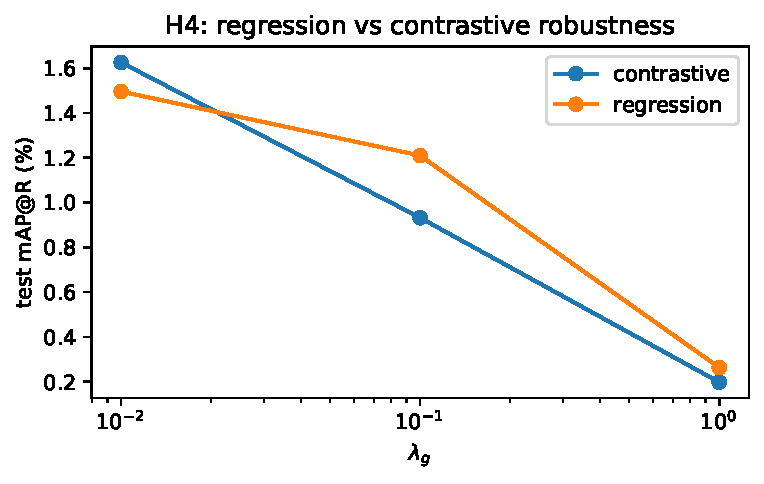
\includegraphics[width=0.6\linewidth]{fig_h4_overlay.pdf}
    \caption{H4: validation mAP@R vs $\lambda_g$ for regression and contrastive.
             Both peak at small $\lambda_g$ and collapse by $\lambda_g{=}1$; no clear
             robustness advantage for contrastive at $n{=}1$.}
    \label{fig:h4}
\end{figure}

\subsection{The \texorpdfstring{$N=3$}{N=3} Comparison against RKD-A}
\label{sec:results-n3}

% ---- GUIDE: N=3 standalone vs RKD-A (H5) ------------------------------------
% HYPOTHESIS H5: at matched arity (order 3), a distance-based graph descriptor
%   transfers comparably/better/worse than RKD-A's angle. RUNS: Graph-RKD N=3 with
%   BOTH descriptors (profile, MDS) vs RKD-A, matched conditions, per (dataset,teacher).
%   ANALYSIS: if RKD-A > Graph-RKD-N3 beyond noise, the angular signal carries
%   information the distance descriptor misses --> motivates angular/hybrid descriptors
%   (future work, Section 10). If comparable/worse, the distance descriptor already
%   captures the triadic structure.
At matched arity ($N{=}3$), Table~\ref{tab:h5} compares Graph-RKD's distance-based
descriptors (profile, MDS) against RKD-A's angle, under identical headline conditions.

\begin{table}[htbp]
    \centering\small
    \caption{H5 --- matched-arity $N{=}3$: median test mAP@R (\%) of Graph-RKD (profile,
             MDS) vs RKD-A, per cell. Cars $n{=}2$--$3$; CUB $n{=}2$ (provisional).}
    \label{tab:h5}
    \begin{tabular}{lccc}
        \toprule
        cell & Graph-RKD (profile) & Graph-RKD (MDS) & RKD-A \\
        \midrule
        Cars / R18 & 3.57 & 3.28 & 1.93 \\
        Cars / CvT & 3.31 & 3.34 & 2.29 \\
        CUB / R18  & 3.31 & 3.03 & 3.50 \\
        CUB / CvT  & 3.13 & 2.98 & 3.07 \\
        \bottomrule
    \end{tabular}
\end{table}

The pattern mirrors the headline. On \textbf{Cars}, the distance descriptor at $N{=}3$
\emph{clearly beats} RKD-A (3.3--3.6 vs 1.9--2.3, both teachers): the triadic distance
structure already carries the useful signal there. On \textbf{CUB}, RKD-A is
competitive --- ahead on ResNet-18 (3.50 vs 3.31 profile / 3.03 MDS) and comparable on
ConvNeXt-Tiny (3.07, straddled by the two descriptors: profile 3.13, MDS 2.98). So on
CUB the \emph{angle} carries information the distance-only descriptor does not fully
capture, which is direct evidence for enriching the graph with angular attributes (a
hybrid distance-plus-angle descriptor) as future work (Section~\ref{sec:conclusion}).
CUB cells are two-seed and provisional.

\subsection{Qualitative Analysis}
\label{sec:results-qual}

% ---- GUIDE: qualitative retrieval panels ------------------------------------
% Produce top-k retrieval panels for representative queries, comparing Graph-RKD
% (best config) against the strongest classic baseline. CAVEAT to retain: queries
% selected by one model's success/failure illustrate ERROR MODES, not the ranking
% (which the tables above quantify). Mark same-class retrievals.
Qualitative top-$k$ retrieval panels --- query images with their nearest neighbours,
same-class hits boxed in green and different-class in red --- are produced by notebook
\texttt{05\_qualitative\_retrieval} from the headline student checkpoints (resolved from
the logged W\&B model artifacts), contrasting Graph-RKD (MDS, $N{=}4$) against the
strongest classic baseline per dataset (triplet-only on Cars, where classic RKD
underperforms; RKD-A on CUB). All four (dataset, teacher) panels are generated; we show
the ResNet-18 cells in Figures~\ref{fig:qual-cars} and~\ref{fig:qual-cub}. The panels are
consistent with the metrics: the Graph-RKD top-1 neighbour is same-class for $25.3\%$ /
$24.6\%$ of Cars queries (ResNet-18 / ConvNeXt-Tiny) and $14.3\%$ / $15.0\%$ of CUB
queries --- matching the logged Recall@1 --- so each panel mixes green (hits) and red
(misses), and the fine-grained error modes are visible directly (same make/model but
wrong instance on Cars; visually similar species on CUB).

\begin{figure}[htbp]
    \centering
    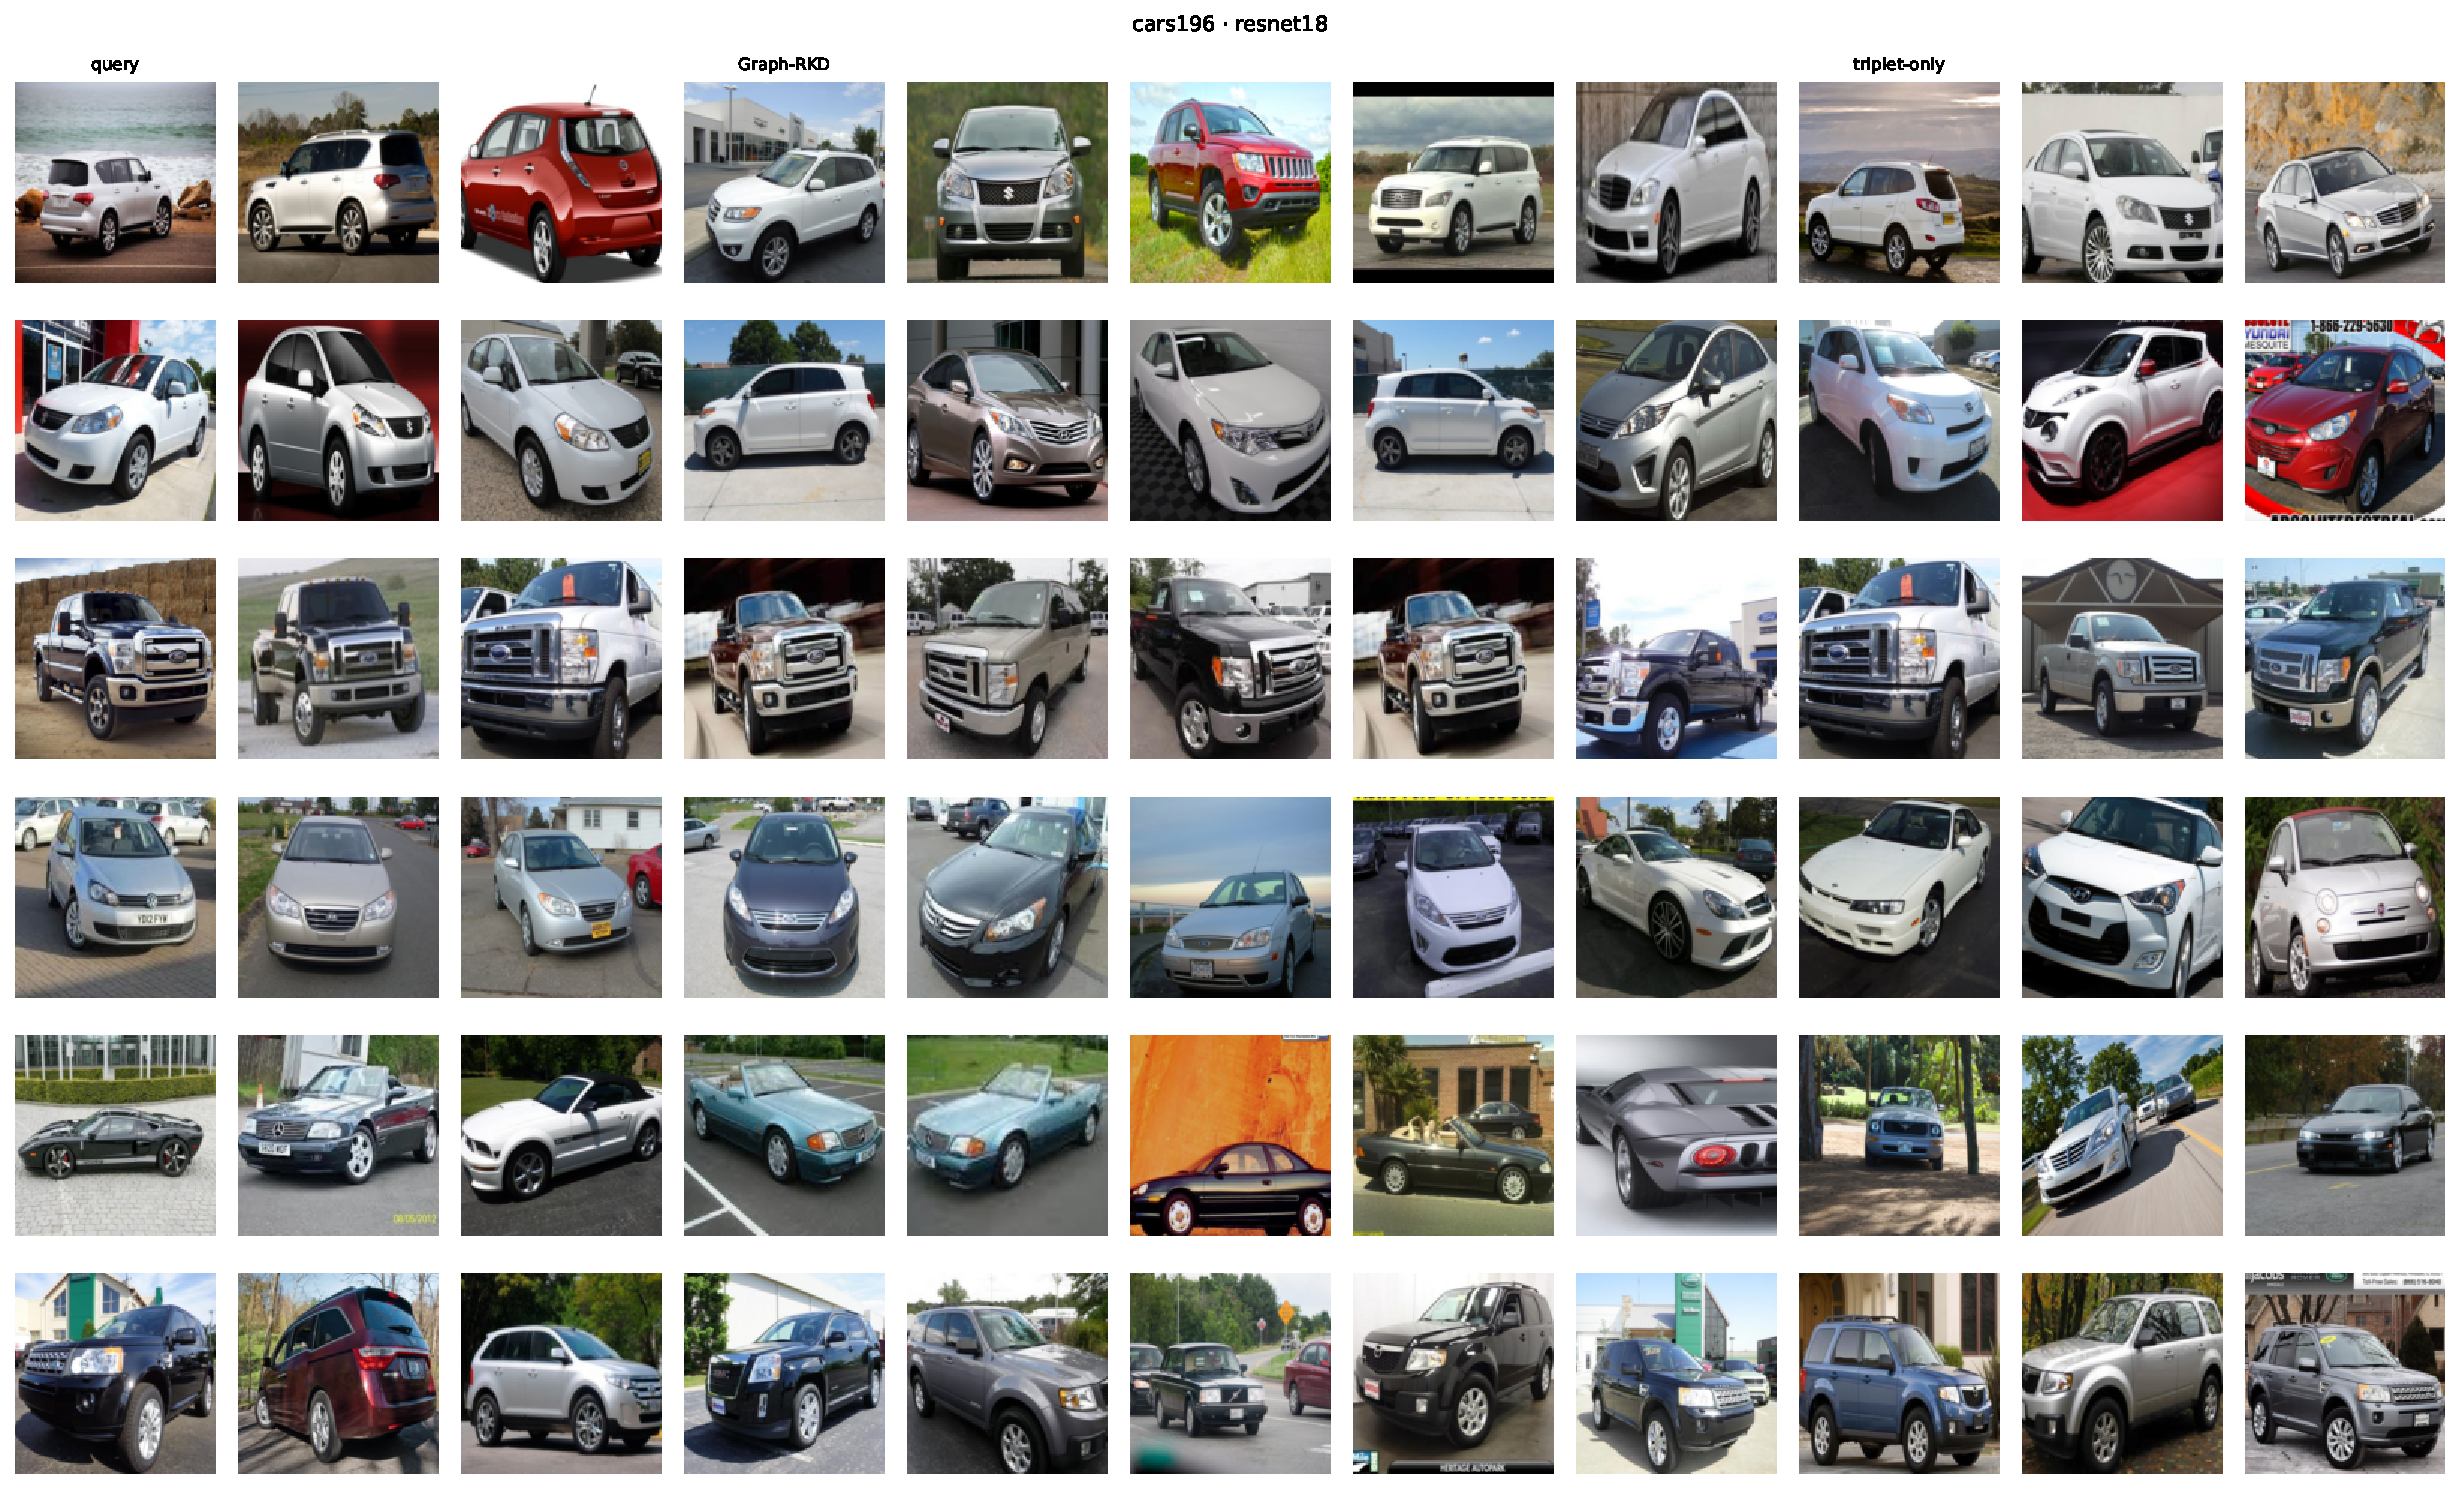
\includegraphics[width=\linewidth]{fig_qual_cars196_resnet18.pdf}
    \caption{Cars-196 / ResNet-18 top-$k$ retrieval. Each row is one query (leftmost
             column); the next five columns are the Graph-RKD nearest neighbours and the
             last five the triplet-only baseline's. Green border $=$ same class, red $=$
             different. Top rows are Graph-RKD top-1 hits, bottom rows its misses.}
    \label{fig:qual-cars}
\end{figure}

\begin{figure}[htbp]
    \centering
    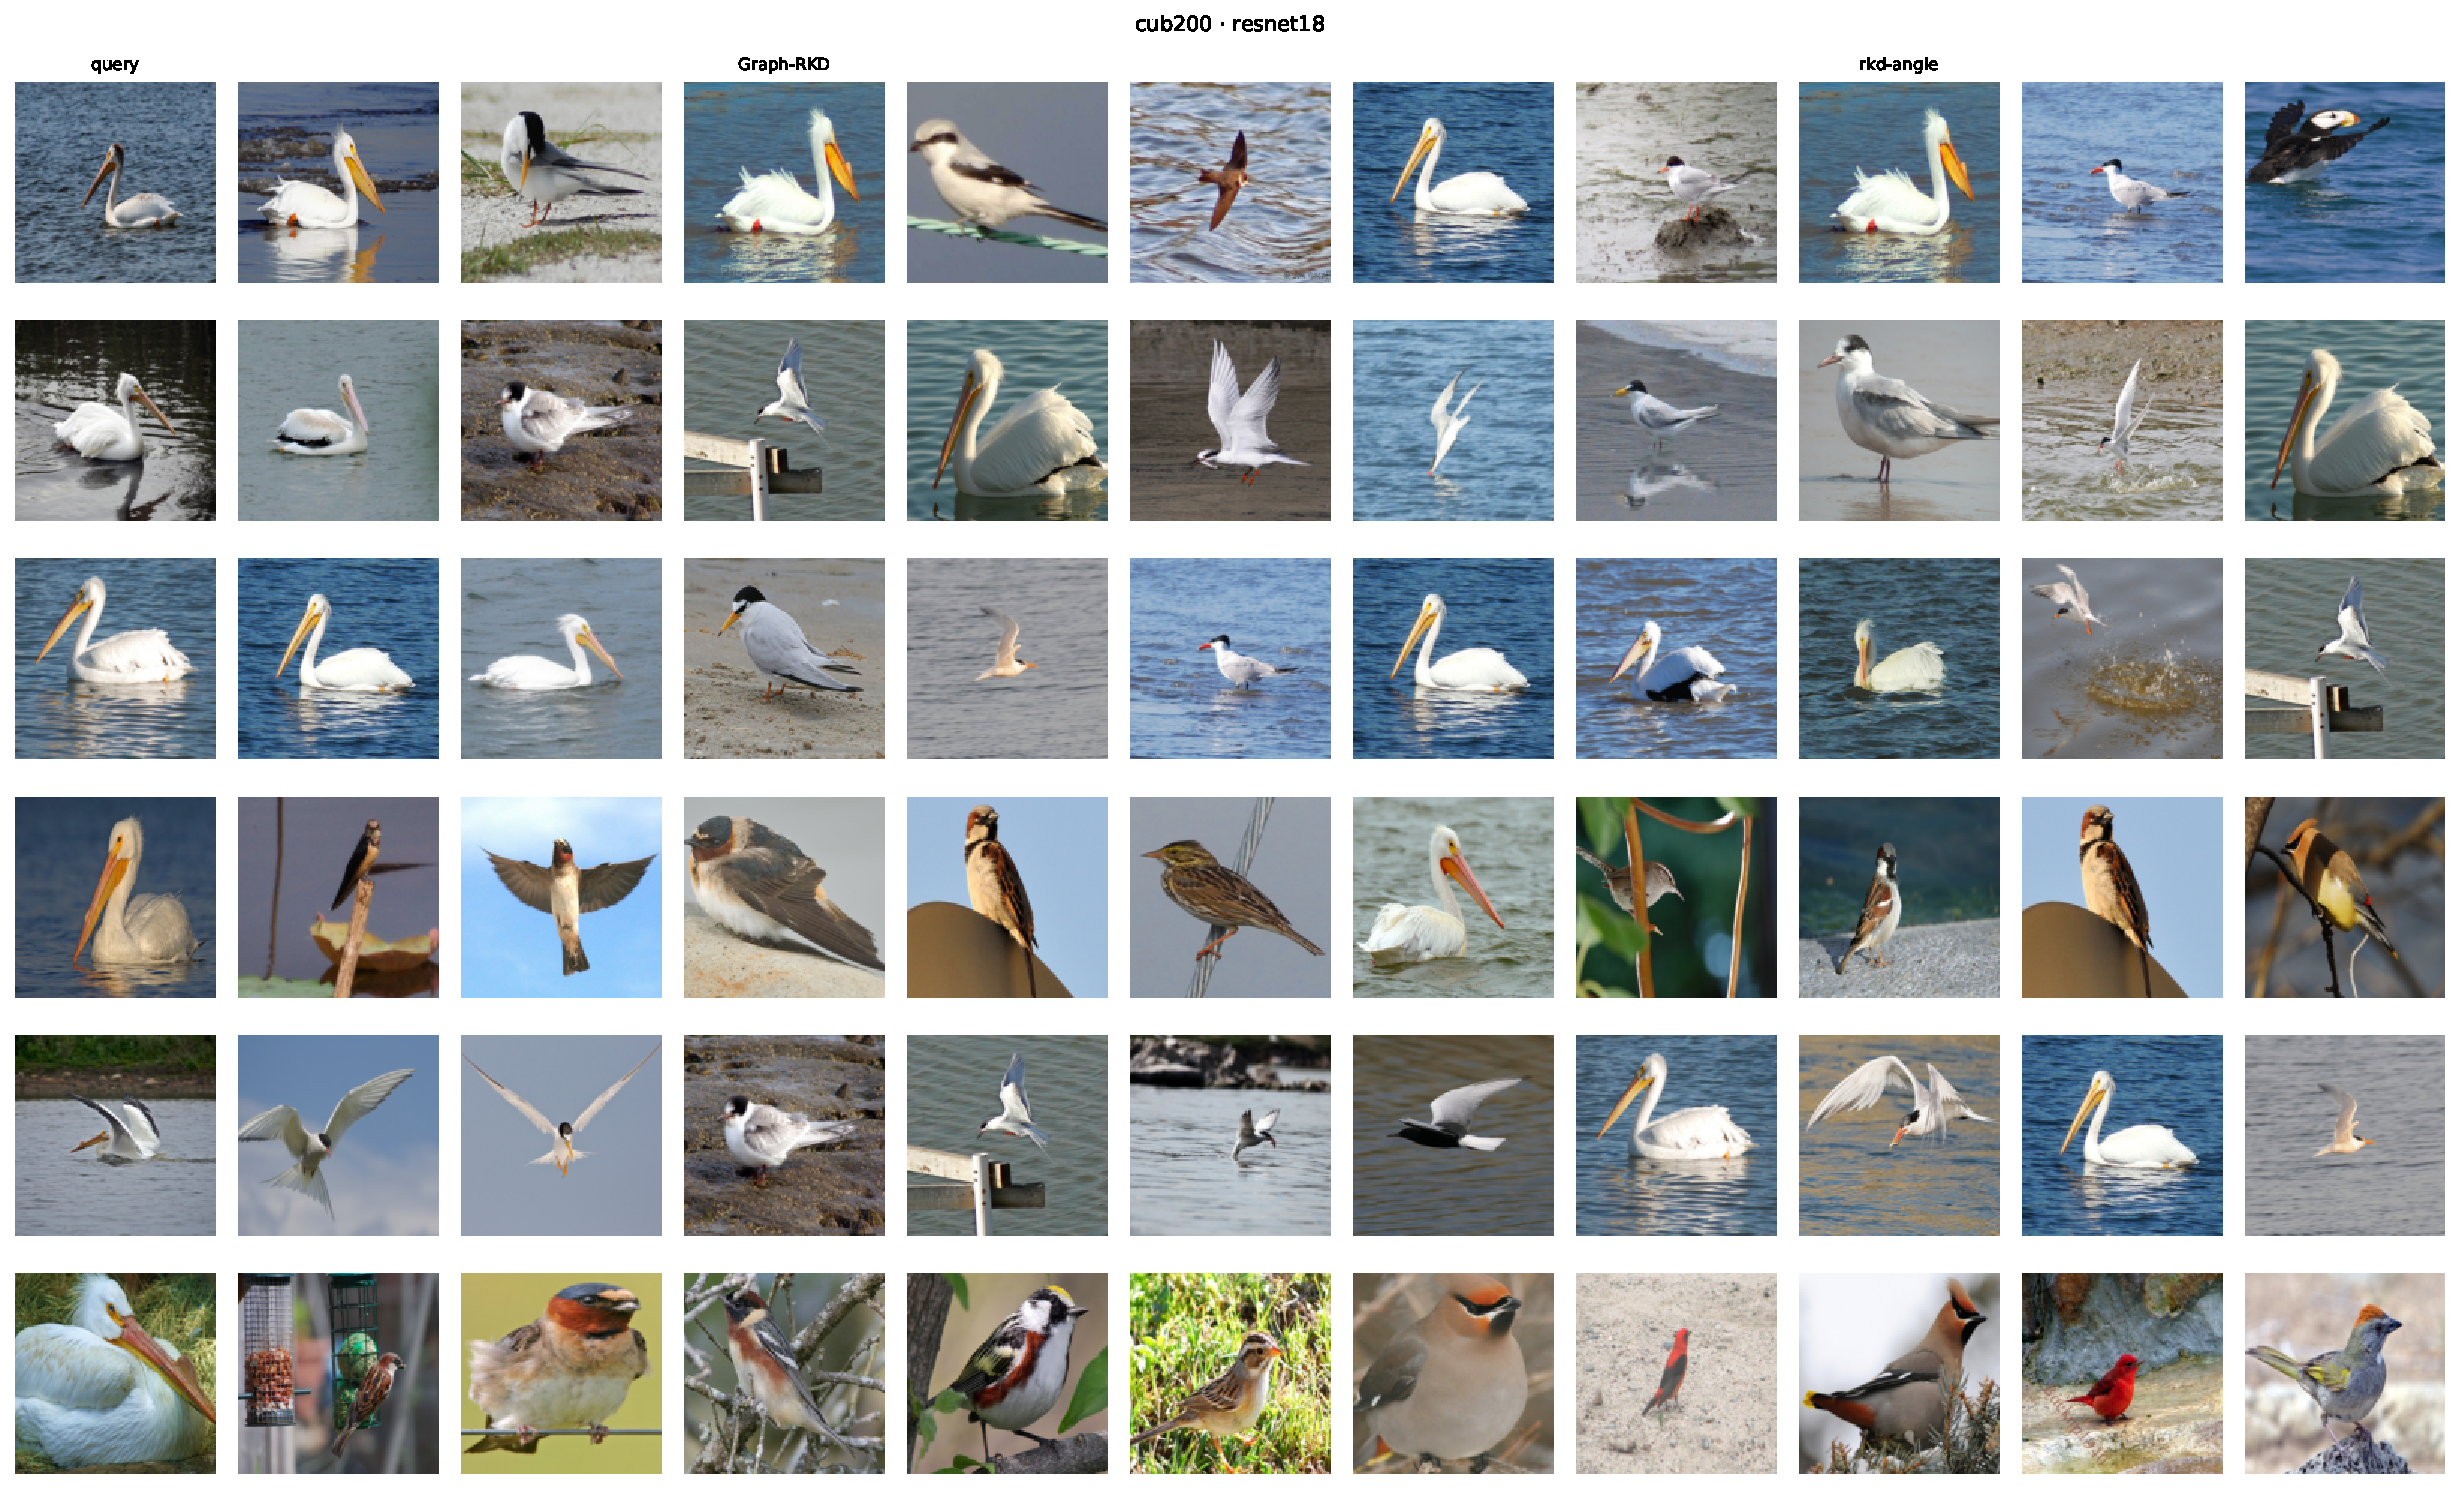
\includegraphics[width=\linewidth]{fig_qual_cub200_resnet18.pdf}
    \caption{CUB-200 / ResNet-18 top-$k$ retrieval: Graph-RKD vs the RKD-A baseline on
             the same queries (same layout as Figure~\ref{fig:qual-cars}). Green $=$ same
             class, red $=$ different.}
    \label{fig:qual-cub}
\end{figure}

\emph{Caveat:} queries chosen by a model's success/failure illustrate error \emph{modes},
not ranking quality --- the latter is quantified by the tables above.

\section{Discussion}
\label{sec:discussion}

Our method is best understood against the evolution of knowledge distillation, whose
progression concerns \emph{what} is taken to constitute the teacher's knowledge:
output logits~\cite{hinton2015distilling}, intermediate feature
maps~\cite{romero2015fitnets}, spatial attention~\cite{zagoruyko2017attention}, and
then the \emph{relations} among examples in Relational KD~\cite{park2019relational}.
Rather than re-narrate that progression (Sections~\ref{sec:introduction}
and~\ref{sec:related}), we position Graph-RKD by what it \emph{subsumes}: modeling a
minibatch as order-invariant graphs generalizes relational transfer to arbitrary
order, and the low orders recover known methods --- $N = 1$ is individual (unary)
distillation, and $N = 2$ is distance-wise RKD (Lemma~\ref{lem:n2}) --- so
$N \geq 3$ is the genuinely new, higher-order regime. In this sense Graph-RKD is a
strict generalization of RKD's own order hierarchy, and the study is framed as a
characterization of its design space (normalization, descriptor, objective) at the
orders where it is a distinct method.

One methodological lesson is worth stating regardless of the empirical outcome: in a
multi-term distillation loss, a term can zero out \emph{silently}. Only per-term
logging (\texttt{train/graph\_loss}) revealed that, under per-graph normalization, the
graph term vanishes identically at $N = 2$; we recommend such monitoring as standard
practice, and it is the reason the normalization axis and Lemma~\ref{lem:n2} are
central to this work rather than an afterthought.

% =============================================================================
%  DISCUSSION OF RESULTS --- TO BE WRITTEN FROM THE RE-RUN EXPERIMENTS.
%
%  The previous discussion drew two conclusions that the revised protocol withdraws
%  as unsupported: (a) "the regression graph term is inert at N=2 and detrimental at
%  every active order" rested on the mis-scaled lambda_g=1000 run, so active orders
%  were never fairly tested; and (b) the "triplet-only vs classic-RKD" collateral
%  finding is out of scope under the reframing. Once the experiments are in, discuss:
%    - Whether Graph-RKD (N>=3) matches/beats RKD-D, RKD-A, combined (the thesis --
%      genuinely undetermined until the runs decide; do not presuppose it).
%    - Which normalization / descriptor / objective wins in which regime.
%    - The N=3 vs RKD-A outcome and whether it motivates angular descriptors.
%    - Teacher-transfer comparison (Q1) on the new numbers.
% =============================================================================

We now read the empirical findings by hypothesis, following the per-cell, range-aware
protocol of Section~\ref{sec:results}. The central outcome is dataset-dependent, and we
treat that sign flip as a result in its own right rather than averaging it away; CUB
cells are two-seed and are discussed as provisional.

% ---- GUIDE: what the completed discussion must cover, by hypothesis ---------
% Write one short paragraph per resolved hypothesis, each stating the verdict AND the
% evidence (with the range-overlap rule and per-cell direction reporting from Section 7):
%   H1 headline: does Graph-RKD (N>=3) match/beat RKD-D, RKD-A, combined? Per
%       (dataset,teacher); discuss any dataset-dependent sign flip explicitly.
%   H2 normalization: which scheme wins at N>=3; did hybrid recover both scale
%       consistency and teacher/student invariance?
%   H3 descriptor: profile vs MDS by regime, tied to the measured stability/fidelity
%       (not raw accuracy alone).
%   H4 objective: is contrastive robust to lambda_g where regression collapses?
%       Report the robust-band width; relate to InfoNCE scale-normalization.
%   H5 (N=3 vs RKD-A): does the result motivate angular descriptors?
%   Q1 (best teacher): state on the new numbers.
% Keep the two paragraphs above (subsumption framing + silent-zero logging lesson) ---
% they survive regardless of outcome.
\textbf{H1 (headline).} Graph-RKD's standing against classic RKD is
\emph{dataset-dependent}, and the flip is the finding, not a nuisance. On Cars-196 the
best-configured Graph-RKD (MDS, $N{=}4$) is the top student on both teachers (3.20 / 3.35
median test mAP@R) while RKD-D, RKD-A and their combination all fall \emph{below} the
triplet-only floor (1.76--2.29 vs 3.07): pairwise distance/angle transfer actively hurts
on Cars, whereas the higher-order graph term helps. On CUB-200 the regime inverts ---
classic RKD helps (RKD-A best, 3.50 / 3.07) and Graph-RKD, though above the floor, does
not exceed the classic variants (it trails RKD-A on ResNet-18 and is level with it on
ConvNeXt-Tiny, where all five students cluster within $\approx$0.1 point). So Graph-RKD
matches-or-beats classic RKD exactly where classic RKD fails, and does not improve on it
where it already works; we make no significance claim on the two-seed CUB cells.

\textbf{H2 (normalization).} Per-graph and minibatch normalization are indistinguishable
at the small orders we use (2.34 vs 2.32 at $N{=}3$), and both clearly beat the
no-normalization variant, whose deficit grows with order as its unnormalized distance
matrices destabilize (none drops from 2.19 at $N{=}3$ to 1.03 at $N{=}8$). The hybrid
scheme did not recover a distinct advantage and was dropped. Normalization is therefore a
genuine design axis --- its absence is harmful and increasingly so with $N$ --- but the
choice between the two viable schemes is immaterial to accuracy; we default to per-graph
for its direct correspondence with classic RKD's distance normalization.

\textbf{H3 (descriptor).} Profile and MDS are equivalent on accuracy across
$N \in \{3,4,8\}$ (within run-to-run noise, MDS marginally ahead at $N{=}3,8$), so no
accuracy-based recommendation is warranted. The separation is on the \emph{mechanism}:
the offline probe shows the MDS spectrum becoming $>$90\% near-degenerate at $N{=}16,17$
(0.1\% at $N{=}3$) while the profile's sort-tie rate grows only mildly. Both are safe at
$N \leq 8$; MDS is our headline descriptor on a razor-thin accuracy edge, and its
large-$N$ fragility is exactly why we do not run MDS at high order.

\textbf{H4 (objective).} The expectation that InfoNCE would be more robust to $\lambda_g$
mis-scaling than regression is \emph{not supported} in our (single-seed) sweep: both peak
at $\lambda_g{=}0.01$ and collapse by $\lambda_g{=}1$, but regression degrades \emph{less}
from $0.01$ to $0.1$ ($-19\%$) than contrastive ($-43\%$). Neither shows a clearly wider
robust band, so we retain regression as the headline objective and flag the robustness
question as needing multiple seeds before any claim.

\textbf{H5 ($N{=}3$ vs RKD-A).} At matched arity, the distance-based graph descriptor
beats RKD-A decisively on Cars (3.3--3.6 vs 1.9--2.3) but not on CUB, where RKD-A is ahead
on ResNet-18 and comparable on ConvNeXt-Tiny. That CUB gap is the clearest actionable
signal in the study: the \emph{angle} RKD-A encodes carries information a distance-only
descriptor misses on that dataset, directly motivating angular or hybrid
distance-plus-angle graph attributes (Section~\ref{sec:conclusion}).

\paragraph{Relation to the project questions (Q1--Q5).}
% TODO: state each project question verbatim before its answer, and note explicitly
% that Q2/Q3/Q4 are answered via a metric-learning reframing (licensed by Q5's
% "adapt to [7]"), since the brief describes a classification setup. Q1 (best
% teacher) depends on the new results; Q2 (post-GAP pooled embedding target, no
% pre-GAP variant for this method), Q3 (no predictor/projection layer needed --
% a strength), Q4 (triplet replaces cross-entropy, graph loss replaces predictor
% MSE), and Q5 (the method IS the RKD adaptation) are framing-level and stable.
\textbf{Q1} (which teacher transfers best): the two teachers differ sharply in their own
retrieval quality (ConvNeXt-Tiny at $36.4$ / $29.3$ test mAP@R on Cars / CUB vs
ResNet-18 at $19.1$ / $18.1$), yet this does \emph{not} translate into proportionally
better students --- distilled students land within $\approx$0.1--0.2 point across
teachers, slightly favouring ConvNeXt-Tiny on Cars and ResNet-18 on CUB. At this
compression teacher \emph{capacity} is not the bottleneck; the transfer signal and the
dataset regime dominate. \textbf{Q2} targets the teacher's post-GAP $L_2$-normalized
pooled embedding (a $192$-, $512$-, and $768$-dimensional space for the student and the
two teachers, bridged with no projection layer). \textbf{Q3} is the $0.67$M-parameter
student (a $16$--$43\times$ reduction). \textbf{Q4} pairs the triplet task loss with the
relational graph loss --- the metric-learning counterpart of the
cross-entropy-plus-regression composition in the brief. \textbf{Q5} is the adaptation of
RKD~\cite{park2019relational} that constitutes the method. We note that the project brief
describes a classification setup, whereas we interpret the task in RKD's native
metric-learning setting; this reframes Q2--Q4 as above and is licensed by Q5's invitation
to adapt to~\cite{park2019relational}.

\section{Difficulties and Solutions}
\label{sec:difficulties}

% =============================================================================
% NOTE: REAL difficulties already encountered + those inherent to the method.
% Fill/adjust as the experiments progress. The ones we know are below.
% =============================================================================

\paragraph{Degenerate normalization at $N = 2$.} The most instructive technical
difficulty was found through per-term logging. Per-graph normalization divides each
distance matrix by the mean of its own off-diagonal entries
(Algorithm~\ref{alg:embedding}), mirroring the classic RKD distance
normalization --- but a two-node graph has a single edge, so the matrix is divided
by itself and every pair of examples maps to the constant matrix
$\bigl[\begin{smallmatrix}0&1\\1&0\end{smallmatrix}\bigr]$, with fixed descriptors
(\texttt{profile} $= (1,1)$; \texttt{mds} eigenvalues $= (0.5, 0)$). Teacher and
student descriptors coincide, and the graph loss and its gradient are identically
zero. The failure is silent: training proceeds normally on the triplet term, and
only the per-term log (\texttt{train/graph\_loss} $= 0$ across all $N = 2$ runs)
exposed it, later confirmed by the derivation of Lemma~\ref{lem:n2} and by direct
execution of the loss code. Rather than a defect to patch after the fact, this
motivated treating normalization as a first-class design axis
(Section~\ref{sec:embeddings}): under minibatch normalization the $N = 2$ descriptor
provably recovers RKD-D (Lemma~\ref{lem:n2}), so we omit $N = 2$ from Graph-RKD
altogether and let the RKD-D baseline represent the pairwise case, evaluating
Graph-RKD only at $N \geq 3$.

\paragraph{Combinatorial growth of higher-order relations.} The number of ordered
$N$-tuples in a minibatch grows super-exponentially with the relational order
(Eq.~\ref{eq:falling_factorial}), which makes a naive higher-order extension of RKD
intractable. We addressed this by modeling each minibatch as order-invariant graphs,
reducing the count to a binomial coefficient (Eq.~\ref{eq:binomial}), and by sampling a
bounded number of graphs per step (Algorithm~\ref{alg:sampling}) so that the per-step
cost is independent of the size of the graph space.

\paragraph{Comparing embedding spaces of different dimensionality.} The teacher and
student produce pooled representations of different widths ($512$ and $768$ for the
teachers, $192$ for the student), so their geometries are not directly comparable. Our
permutation-invariant graph descriptors have a dimensionality that depends only on the
relational order $N$, not on the representation width, so teacher and student
embeddings inhabit the same descriptor space and require no projection layer;
normalizing the distance matrix (under any of the schemes studied) further removes
scale mismatch.

\paragraph{Preserving per-example correspondence.} The graph loss must pair the student
and teacher on identical node sets. This rules out augmentations that mix samples, such
as mixup and cutmix, which would break the correspondence; we therefore exclude them
from the distillation runs (Section~\ref{sec:preprocessing}). This choice also means the
teacher's embeddings cannot be precomputed and cached (each epoch's augmentation changes
them); within a step, however, the $K \times K$ teacher distance matrix is computed once
and sliced for the sampled graphs.

\paragraph{Experiment organization and resources.} Studying normalization, descriptor,
objective, and order jointly yields a large configuration grid; managing, tuning
($\lambda_g$ per configuration), and analyzing it under limited time and compute
required staging the runs (establishing active-order viability on a targeted slice
before expanding) and using targeted comparisons rather than the full cross-product.
The campaign is enumerated once as independent per-experiment jobs and executed through
whichever backend was available: cheap iteration on rented serverless GPUs (no quota),
and the full run on a single local GPU packing several jobs per card. A managed
cloud-training backend was also implemented but could not be used --- its GPU quota was
declined for a new account --- which is itself a practical lesson: quota, not code, was
the binding constraint, and decoupling the plan from any single backend was what kept
the study runnable.
% [Add here any training-stability or dataset-specific issues encountered during the
%  actual runs, e.g. convergence behavior on CUB-200 vs Cars-196, memory pressure at
%  large N, temperature sensitivity in the contrastive objective.]

\section{Conclusion and Future Work}
\label{sec:conclusion}

This work asked whether Relational Knowledge Distillation can be generalized beyond
pairs and triplets, and how the resulting method compares to RKD at the orders where
it is distinct. We proposed Graph-RKD, which models each minibatch as complete,
undirected, weighted graphs over its examples; summarizes every graph with a
permutation-invariant descriptor (sorted node profiles or the classical-MDS spectrum);
keeps the loss tractable by sampling a bounded, adaptively sized set of graphs at each
step; and studies three design axes --- normalization, descriptor, and objective ---
comparing Graph-RKD at $N \geq 3$ against the RKD-D and RKD-A baselines under a shared,
fair protocol. The formulation reduces the space of order-$N$ relations from a falling
factorial to a binomial coefficient and, because descriptor dimensionality depends only
on $N$, requires no projection layer between teacher and student spaces. Analytically,
we showed (Lemma~\ref{lem:n2}) that the pairwise case $N = 2$ either degenerates or
reduces exactly to RKD-D, so Graph-RKD recovers RKD's low orders as special cases and
is a strict higher-order generalization.

% =============================================================================
%  CONCLUSION OF RESULTS --- TO BE COMPLETED FROM THE RE-RUN EXPERIMENTS.
%  Do not state a negative or positive headline until the fair, re-tuned, multi-seed
%  comparison (Graph-RKD N>=3 vs RKD-D/RKD-A) is complete. The earlier "negative
%  result" framing was withdrawn because active orders were never fairly tested
%  (mis-scaled lambda_g) and N=2 was degenerate.
% =============================================================================

Empirically, the answer is dataset-dependent. On Cars-196 the best-configured Graph-RKD
($N{=}4$, MDS, per-graph, regression) is the strongest student on both teachers and, in
those same cells, classic pairwise RKD falls below the triplet-only floor --- the
higher-order graph term succeeds precisely where distance/angle RKD fails. On CUB-200 the
opposite holds: classic RKD helps and Graph-RKD, while above the floor, does not surpass
it (two-seed, provisional). Along the design axes, normalization is a genuine axis
(per-graph $\approx$ minibatch $\gg$ none, the gap widening with $N$); the two descriptors
are accuracy-equivalent at $N \leq 8$ and separated only by MDS's large-$N$ degeneracy;
and the $\lambda_g$-robustness advantage we expected of the contrastive objective did not
materialize at single seed. The matched-arity comparison ($N{=}3$ vs RKD-A) yields the one
sharp prescription: distance-based graphs already dominate on Cars but leave an angular gap
on CUB. We therefore report Graph-RKD as a viable higher-order generalization of RKD whose
benefit is \emph{regime-dependent} rather than a uniform win --- a characterization offered
with the explicit caveat that the CUB cells rest on two seeds.

The principal direction for future work is a rule $N^\ast(K)$ predicting the
quality-optimal relational order from the minibatch size, which would require sweeping
$K$ across datasets, teachers, descriptors, objectives, and normalization schemes --- a
study in its own right, for which the fixed-$K$ per-order characterization here is the
groundwork. A second direction, motivated by RKD-A's angular relation, is to enrich the
graphs with angular attributes (e.g.\ per-node angular profiles or a hybrid
distance-plus-angle descriptor), bringing the information exploited by RKD-A into the
graph formulation and subsuming both RKD-D and RKD-A as low-order special cases within a
single descriptor.

\section*{Use of AI Assistance}
\label{sec:ai-assistance}

We used Claude Code (Anthropic) as an assistant tool throughout this project: for
writing and refactoring code (the training pipeline, the graph-descriptor and loss
implementations, the experiment-orchestration and analysis tooling), for drafting and
editing this manuscript, and for general idea generation and problem solving (e.g.\
shaping the experimental protocol, debugging, and reasoning through design trade-offs).
All research decisions, the experimental design, and the interpretation of results
remain the authors' own; the authors reviewed and are responsible for all code,
text, and claims presented here.

% =============================================================================
%  REFERENCES
% =============================================================================
\bibliographystyle{ieeetr}
\bibliography{references}

\end{document}

% =============================================================================
%  REUSABLE SNIPPETS  (uncomment and paste where needed)
% =============================================================================
%
% --- FIGURE WITH IMAGE FILE --------------------------------------------------
% \begin{figure}[h]
%     \centering
%     \includegraphics[width=0.7\textwidth]{path/figure.png}
%     \caption{Caption explaining the figure.}
%     \label{fig:my-figure}
% \end{figure}
% Reference it as: Figure~\ref{fig:my-figure}
%
% --- SUBFIGURES --------------------------------------------------------------
% \begin{figure}[h]
%     \centering
%     \begin{subfigure}[b]{0.45\textwidth}
%         \includegraphics[width=\textwidth]{path/left.png}
%         \caption{Left panel.}
%         \label{fig:left}
%     \end{subfigure}\hfill
%     \begin{subfigure}[b]{0.45\textwidth}
%         \includegraphics[width=\textwidth]{path/right.png}
%         \caption{Right panel.}
%         \label{fig:right}
%     \end{subfigure}
%     \caption{Combined caption.}
%     \label{fig:combo}
% \end{figure}
%
% --- NUMBERED EQUATION -------------------------------------------------------
% \begin{equation}
%     \mathcal{L} = \alpha \, \mathcal{L}_{MSE} + (1-\alpha) \, \mathcal{L}_{CE}
%     \label{eq:my-eq}
% \end{equation}
% Reference it as: Equation~\ref{eq:my-eq}
%
% --- CITATION ----------------------------------------------------------------
% Single:  \cite{hinton2015distilling}
% Multiple: \cite{hinton2015distilling,romero2015fitnets,zagoruyko2017attention}
%
% =============================================================================
